\documentclass[12pt]{article}
\usepackage[utf8]{inputenc}
\usepackage[russian]{babel}
\usepackage{graphicx}
\usepackage{amsmath}
\usepackage{hyperref}
\usepackage{algorithm}
\usepackage{cmap}  
\usepackage{epstopdf}
\usepackage[noend]{algorithmic}

\textheight = 24.5cm
\textwidth = 17cm
\oddsidemargin = 0pt
\topmargin = -2.2cm
\parskip = 5pt
\tolerance = 2000
\hyphenpenalty = 10


\def\algorithmicrequire{\textbf{Вход:}}
\def\algorithmicensure{\textbf{Выход:}}
\def\algorithmicif{\textbf{если}}
\def\algorithmicthen{\textbf{то}}
\def\algorithmicelse{\textbf{иначе}}
\def\algorithmicelsif{\textbf{иначе если}}
\def\algorithmicfor{\textbf{для}}
\def\algorithmicforall{\textbf{для всех}}
\def\algorithmicdo{\textbf{выполнять}}
\def\algorithmicwhile{\textbf{пока}}
\def\algorithmicrepeat{\textbf{повторять}}
\def\algorithmicuntil{\textbf{пока}}
\def\algorithmicloop{\textbf{цикл}}
\def\algorithmiccomment#1{\quad// {\sl #1}}


\begin{document}

\begin{center}
\thispagestyle{empty}
Московский Государственный Университет им. М.В. Ломоносова

\begin{figure}[h!]
\begin{center}
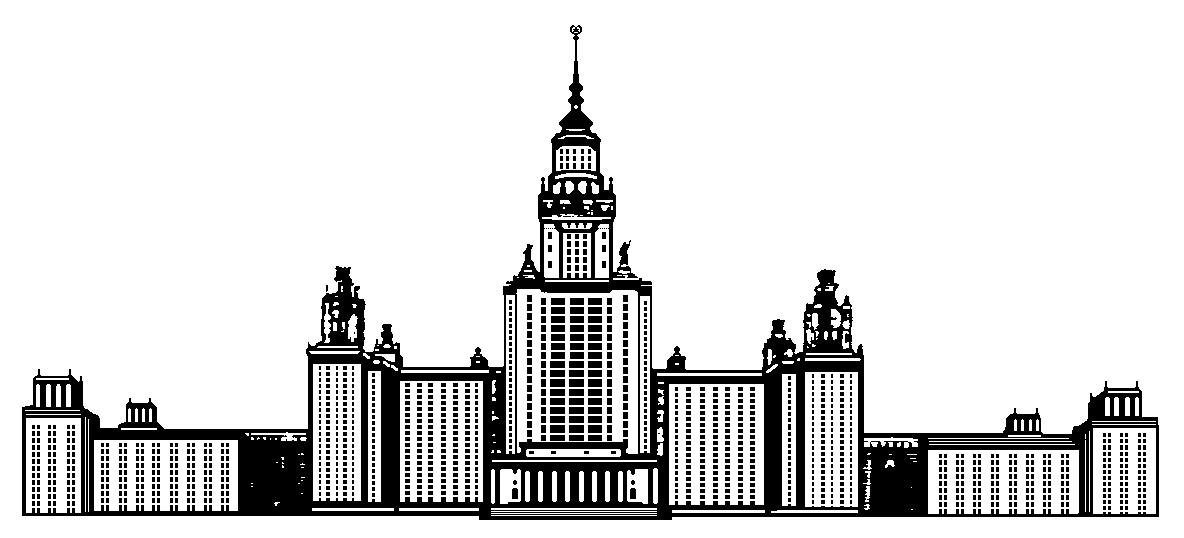
\includegraphics[scale = 0.1]{title_image.png}
\end{center}
\end{figure}

Факультет Вычислительной Математики и Кибернетики

Кафедра Математических Методов Прогнозирования

\vspace{88pt}
\large

\LARGE
{\bf Курсовая работа}
\vspace{20pt}

{\bf <<Регуляризация тематических моделей в библиотеке BigARTM>>}

\vspace{120pt}
\begin{flushright}
\normalsize

\hfill\parbox{8cm}{
Выполнил:

\vspace{5pt}
студент 3 курса 317 группы

\vspace{5pt}
{\it Апишев~Мурат~Азаматович}

\vspace{20pt}
Научный руководитель:

\vspace{5pt}
д.ф-м.н., доцент

\vspace{5pt}
{\it Воронцов~Константин~Вячеславович.}
}

\vspace{80pt}
\center{Москва, 2014}
\end{flushright}

\newpage
\end{center}

\tableofcontents
\newpage

\section{Введение}\label{introduction}

$\quad\;\:$Тематическое моделирование --- активно развивающаяся в последние годы область машинного обучения. Оно позволяет решать задачи тематического поиска, категоризации и кластеризации корпусов текстовых документов. Аналогичные задачи решаются для коллекций изображений и видеозаписей.

Тематическая модель определяет, к каким темам относится каждый документ, а также то, какие термины из словаря образуют ту или иную тему.

В работе \cite{voron2014} предлагается полувероятностный подход к тематическому моделированию --- аддитивная регуляризация тематических моделей (АРТМ). Он позволяет записать любое количество дополнительных требований к тематической модели в виде взвешенной суммы критериев, добавляемых к основному функционалу логарифмированного правдоподобия. В \cite{voron2014} показано, что многие известные тематические модели допускают такое представление, то есть фактически являются лишь формой регуляризации. При этом, в отличие от стандартных задач машинного обучения --- классификации и регрессии, в тематическом моделировании возникает огромное разнообразие регуляризаторов, направленных на улучшение модели и учёт дополнительной информации о текстовой коллекции. Задача тематического моделирования является по сути многокритериальной, и АРТМ позволяет выразить это непосредственным образом. Более распространённый в литературе байесовский подход основан на гипотезе о существовании адекватной вероятностной модели порождения текста. Эта гипотеза представляется избыточно сильной, так как далеко не все лингвистические требования и знания о естественном языке допускают вероятностую трактовку. Кроме того, техника байесовского вывода, как показывают работы последних лет, создаёт большое число технических трудностей при построении комбинированных моделей и попытках одновременного учёта большого числа разнородных требований.

Благодаря АРТМ появляется новая возможность --- создать библиотеку из десятков различных регуляризаторов и строить решения прикладных задач путём обоснованного выбора  подмножества регуляризаторов. В данной курсовой работе рассматривается архитектура и отдельные элементы библиотеки BigARTM, в которой в настоящее время реализуется данная концепция. Особое внимание уделяется мультипроцессорному и кластерному распараллеливанию, поскольку библиотека BigARTM изначально проектируется для тематического моделирования больших коллекций.   

Работа имеет следующую структуру: в разделе \ref{defenitions} введены базовые обозначения и определения, необходимые для дальнейшего изложения; алгоритм обучения тематических моделей и идея регуляризации вводятся в разделе \ref{learning}; в разделе \ref{overview} приводится краткий обзор существующих параллельных библиотек тематического моделирования; раздел \ref{library} описывает общую архитектуру библиотеки и схему пользовательского взаимодействия с BigARTM; раздел \ref{regularizers} посвящён реализации и использованию регуляризаторов в библиотеке; в \ref{experiments} разделе показаны эксперименты с регуляризаторами; раздел \ref{results} предназначен для выводов и подведения итогов курсовой работы.

\section{Терминология}\label{defenitions}

Прежде всего рассмотрим некоторые базовые понятия и необходимые обозначения.

Вероятностная тематическая модель (ВТМ) описывает каждую тему дискретным распределением на множестве терминов, каждый документ --- дискретным распределением на множестве тем. Предполагается, что коллекция документов --- это последовательность терминов, выбранных случайно и независимо из смеси таких распределений, и ставится задача восстановления компонент смеси по выборке.

\begin{itemize}
	\item $D$ --- коллекция текстовых документов.
	\item $W$ --- словарь коллекции текстов.
	\item $T$ --- множество тем.
\end{itemize}

Документы в коллекции можно представить в виде так называемого <<мешка слов>>. В рамках этой концепции документ рассматривается как множество терминов из словаря и соответствующих им счётчиков частот встречаемости.

{\bf Замечание: } <<Мешок слов>> на данный момент является основным способом представления коллекции, однако в последнее время всё большее развитие получают идеи хранения документа в виде последовательности слов. Порядок слов при этом становится важным и используется для улучшения качества обучения модели. BigARTM будет поддерживать оба способа представления.

После принятия гипотезы <<мешка слов>>, коллекция представляется в виде матрицы $F_{W \times D}$, строки которой соответствуют терминам из словаря, а столбцы --- документам коллекции. На пересечении строки и столбца находится оценка вероятности встретить данное слово в данном документе. Эта оценка является отношением числа раз, которое слово встретилось в документе, к общему числу слов в этом документе. Таким образом, столбцы матрицы $F$ представляют собой распределения вероятностей.

При рассмотрении коллекции в виде пар $(d, w)$, где $w$ --- номер термина, а $d$ --- номер документа, вводятся следующие счётчики частот:

\begin{itemize}
	\item $n_{dw}$ --- число вхождений термина $w$ в документ $d$;
	\item $n_d = \sum_{w \in W} n_{dw}$ --- длина документа $d$ в терминах;
	\item $n_w = \sum_{d \in D} n_{dw}$ --- число вхожденией документа $w$ во все документы коллекции;
	\item $n = \sum_{d \in D}\sum_{w \in d} n_{dw}$ --- длина коллекции $D$ в терминах; 
\end{itemize}

Если же рассматривать коллекцию в виде троек $(d, w, t)$, где $d$, $w$ и $t$ --- номера соответствующих документа, термина и темы, то можно ввести такие счётчики: 

\begin{itemize}
	\item $n_{dwt}$ --- число троек, в которых термин $w$ встретился в документе $d$ и связан с темой~$t$;
	\item $n_{dt} = \sum_{w \in W} n_{dwt}$ --- число троек, в которых термин из документа $d$ связан с темой $t$;
	\item $n_{wt} = \sum_{d \in D} n_{dwt}$ --- число троек, в которых термин $w$ связан с темой $t$;
	\item $n_t = \sum_{d \in D}\sum_{w \in d} n_{dwt}$ --- число троек, связанных с темой $t$;
\end{itemize}

С использованием данных счётчиков можно ввести следующие частотные оценки вероятностей, связанных со скрытой переменной $t$:

\begin{itemize}\label{label_1}
\item $ 
	\hat p(w|t) = \cfrac{n_{wt}}{n_t}, \quad
	\hat p(t|d) = \cfrac{n_{dt}}{n_d}, $ 
\end{itemize}

Ставится задача разложения матрицы $F$ в произведение двух матриц $\Phi$ и $\Theta$ меньшего размера, таких, что

\begin{itemize}
\item $\Phi = (\phi_{wt})_{W \times T}, \; \phi_{wt} = \hat p(w|t)$ --- матрица <<термины-темы>>;
\item $\Theta = (\theta_{td})_{T \times D}, \; \theta_{td} = \hat p(t|d)$ --- матрица <<темы-документы>>;
\end{itemize}

Поставленная задача ($F \approx \Phi \Theta$) эквивалентна поиску матриц $\Phi$ и $\Theta$, максимизирующих следующий функционал правдоподобия:

\begin{equation}\label{eq_1}
 	L(\Phi, \Theta) = \sum_{d \in D} \sum_{w \in d} n_{dw} \sum_{t \in T} \phi_{wt} \theta_{td} \rightarrow \max_{\Phi, \Theta}
\end{equation}


\section{Обучение тематических моделей}\label{learning}

\subsection{PLSA}

Вероятностный латентный семантический анализ (PLSA) был предложен Т.Хофманном в~\cite{hofmann_plsa}.

Примем гипотезу условной независимости, утверждающую, что вероятность появления термина в данном документе зависит только от темы этого термина и не зависит от документа. Вероятностная порождающая модель PLSA имеет следующий вид: 
\[
	p(w|d) = \sum_{t \in T} p(w|t) p(t|d)
\]

PLSA можно реализовать с помощью ЕМ-алгоритма. Итерационный процесс состоит из двух шагов --- Е-шага (Expectation) и М-шага (Maximization). На Е-шаге по текущим значениям $\phi_{wt}$ и $\theta_{td}$ c помощью формулы Байеса вычисляются условные вероятности $p(t|d,w)$:
\[
	H_{dwt} = p(t|d,w) = \cfrac{\phi_{wt}\theta_{td}}{\sum_{s \in T}\phi_{ws}\theta_{sd}}
\]

На М-шаге по условным вероятностям $H_{dwt}$ вычисляются новые приближения параметров $\phi_{wt}$ и $\theta_{td}$. Используются указанные в предыдущем разделе формулы:
\[
	\phi_{wt} = \cfrac{n_{wt}}{n_t}, \quad
	\theta_{td} = \cfrac{n_{dt}}{n_d}, \quad	
\]

\subsection{Аддитивная регуляризация}

Неоднозначность матричного разложения $F \approx \Theta \Phi$ даёт свободу выбора матриц из правой части равенства, позволяя наложить на тематическую модель дополнительные требования.  
Модифицируем максимизируемый функционал \ref{eq_1}:

\begin{equation}
	\quad L(\Phi,\Theta) + R(\Phi,\Theta) \rightarrow \max_{\Phi,\Theta}
\end{equation}	


\[
 	R(\Phi,\Theta) = \sum_{i = 1}^{n} \tau_i R_i(\Phi,\Theta)
\]	
где $R_i(\Phi,\Theta)$ --- дополнительные требования к модели, $\tau_i$ --- неотрицательные  коэффициенты регуляризации, выполнены условия неотрицательности и нормировки столбцов матриц $\Phi$ и $\Theta$.
 	 
Решение этой задачи приводит к обощению формул М-шага в ЕМ-алгоритме:
\begin{equation}
	\phi_{wt} = \cfrac{\left(n_{wt} + \phi_{wt} \cfrac{\partial R}{\partial \phi_{wt}} (\Phi,\Theta) \right)_+}{\sum_{u \in W} \left(n_{ut} + \phi_{ut} \cfrac{\partial R}{\partial \phi_{ut}} (\Phi,\Theta) \right)_+}, \quad 
 	\theta_{td} = \cfrac{\left(n_{dt} + \theta_{td} \cfrac{\partial R}{\partial \theta_{td}} (\Phi,\Theta) \right)_+}{\sum_{s \in T} \left(n_{ds} + \theta_{sd} \cfrac{\partial R}{\partial \theta_{sd}} (\Phi,\Theta) \right)_+}
\end{equation} 
 	 
 	 $n_{wt}$ и $n_{dt}$ определяются аналогично из формул предыдущего раздела.
 	 
Таким образом, суть добавления регуляризаторов --- в простом изменении формул М-шага.

{\bf Замечание:} Использование регуляризаторов требует аккуратного выстраивания т.н. траектории регуляризации. Этот процесс включает в себя настройку параметров, определение времени подключения/отключения того или иного регуляризатора, используемого в модели и т.п.

\section{Существующие реализации параллельных алгоритмов}\label{overview}

В данном разделе кратко рассматриваются некоторые известные параллельные алгоритмы тематического моделирования. Все они основаны на модели LDA, имеют разные технические и алгоритмические детали. Рассмотрим их основные преимущества и недостатки, после чего опишем на основе полученных выводов основные требования к BigARTM. 

\subsection{Краткий обзор}

\paragraph{AD-LDA}
Данный алгоритм был предложен в работе \cite{ad_lda}. В AD-LDA был реализован только межпроцессорный параллелизм, возможность работы на кластере не обсуждалась. 

Представленная архитектура предпологает размещение документов в случайном порядке на каждом из участвующих в вычислениях процессоров. Все процессоры одновременно производят сэмплирование, получая счётчики матрицы $\Theta$. Этот процесс происходит до тех пор, пока все процессоры не закончат работу. После производится шаг синхронизации, на котором счётчики со всех процессоров сливаются вместе. Затем происходит обновление глобальной матрицы $\Phi$. Новая $\Phi$ рассылается каждому процессору, и начинается следующая итерация симплирования. И так до тех пор, пока не выполнится заданный критерий останова.

Данная работа является одной из первых, в которых была осознана возможность параллелизации процеса обучения модели, и в этом её серьёзное достоинство. Но сама реализация имеет ряд серьёзных недостатков:

\begin{enumerate}
	\item Скорость работы алгоритма определяется скоростью самого медленного процессора.
	\item Нагрузка на сеть неравномерная --- высока во время синхронизации и почти нулевая во время сэмплирования. 
	\item Система обладает низкой отказоустойчивостью.
	\item Наличие отдельной матрицы $\Phi$ у каждого процессора приводит к большим затратам памяти.
\end{enumerate}

Как видно, большинство недостатков возникают как следствие наличия отдельного шага синхронизации.

\paragraph{PLDA}
PLDA был описан в статье \cite{plda}. Алгоритм представляет собой модификацию AD-LDA, в которой параллелизм реализован в двух вариантах: с помощью MPI и Map-Reduce (при этом работа опять же распределяется между процессорами, кластерная реализация отсутствует). 

Архитектура не претерпела больших изменений. Существенной модификацией является использование контрольных точек --- откачки данных после очередной итерации сэмплирования на жёсткий диск. В случае сбоя имеется возможность восстановить данные и продолжить вычисления. В MPI-реализации это действительно работает хорошо. В Map-Reduce версии реализация контрольных точек требует больших затрат памяти. Авторы сами рекомендуют использовать MPI.

Собственно, помимо низкой отказоустойчивости, PLDA сохранил все недостатки AD-LDA.

\paragraph{Y!LDA}
Следующим шагом для параллельных алгоритмов обучения тематических стала работа Y!LDA, описанная в \cite{y_lda}. Авторы рассмотрели недостатки AD-LDA и предложили свой вариант параллелизма, теперь уже как в рамках одной машины, так и в кластере. Основным достижением стало избавление от выделенного шага синхронизации. Авторы отметили его основные недостатки (плохая отказоустойчивость, неравномерная нагрузка на сеть и ожидание медленных процессоров) 
и предложили способ избавления от них, который будет рассмотрен далее.

Коллекция делится между машинами. В свою очередь, в рамках каждой ноды документы распределяются по процессорам. Все процессоры одного компьютера имеют общую матрицу $\Phi$, что существенно снижает затраты памяти. На каждой ноде имеется т.н. поток синхронизации, к которому ядра обращаются независимо по мере завершения обработки очередной порции документов.

Глобальная матрица $\Phi$ хранится в \verb|memcached|
\footnote{memcached — связующее программное обеспечение, реализующее сервис кэширования данных в оперативной памяти на основе парадигмы хеш-таблицы.}.
.
Работа кластера организована с использованием т.н. <<архитектуры классной доски>>. Суть её состоит в том, что каждый компьютер в сети обращается к глобальной матрице $\Phi$ независимо от других, обновляя полученные им счётчики. Порцией обновления при этом является один термин. Кластерный параллелизм был реализован в Hadoop.

\paragraph{PLDA+}
В публикации \cite{plda_plus} была предпринята попытка модифицировать PLDA. Авторы сделали алгоритм параллельным в кластерном смысле. Для того, чтобы побороть проблемы, связанные с шагом синхронизации, было решено использовать конвейерную архитектуру. Для этого всё множество процессоров делитя на две группы --- вычислители и коммутаторы. Первая группа производит сэмплирование (собственно расчёт модели), вторая отвечает за своевременную доставку данных. Вкупе с равномерным распределением коллекции в виде блоков по процессорам-вычислителям, а также наличием механизма приоритетов, сглаживающем узкие места во время счёта, это даёт, согласно экспериментам, хорошие результаты. Тем не менее, один существенный недостаток у данной реализации имеется --- значимая часть вычислительных ресурсов тратится не на счёт, а на своевременную доставку данных.

\subsection{BigARTM}
Из всего вышеописанного были сделаны нижеследующие выводы:

\begin{enumerate}
	\item Алгоритм обязательно должен быть асинхронным, что позволит избежать недостатки AD-LDA.
	\item Матрица $\Phi$ должна быть локальной в рамках компьютера, а не ядра, что приведёт к существенной экономии оперативной памяти.
	\item Использование \verb|memcached| является хорошим решением для хранения глобальной матрицы $\Phi$
	\footnote{К сожалению, сервис memcached предназначен для использования только под Linux. Тем не менее, это не является большой проблемой, поскольку большинство кластеров работает именно под Unix-подобными ОС и кластерный параллелизм BigARTM будет ориенторован именно под них. Windows-версия библиотеки, по сути, предназначена для использования на локальной машине. Хотя, возможно, к релизу для Windows-версии будет написан сервис, осуществляющий функции memcached, как это уже сделано в рамках многопроцессорного параллелизма.}
	.
	\item Коллекцию следует разделить на пакеты документов, обрабатываемых независимо.
\end{enumerate}

Все эти идеи положены в основу BigARTM. Они либо уже реализованы, либо будут реализованы к моменту релиза библиотеки.
Таким образом, BigARTM архитектурно похож на Y!LDA, за исключением использованного фреймворка для организации кластерного параллелизма (MPI вместо Hadoop).

\section{Библиотека BigARTM}\label{library}
BigARTM --- библиотека тематического моделирования, реализующая концепцию аддитивной регуляризации. На данный момент библиотека поддерживает многопроцессорный параллелизм. Основным алгоритмом является описанный в \ref{plsa_alg} Online Batch PLSA.

\paragraph{Protocol buffers}
\footnote{Подробнее о том, что такое Google Protocol Buffers и как с ними работать, можно прочесть в \cite{protobuf}}
Рассмотрим кратко эту технологию, поскольку в BigARTM она используется очень интенсивно. Protocol Buffers позволяет описывать proto-сообщения на псевдоязыке, которые затем можно преобразовать специальным компилятором (protoc) в структуры данных со всеми необходимыми методами на С++, Python и Java. Ключевой особенностью является возможность обмена сообщениями между этими языками программирования посредством механизма serializer/deserializer, переводящего сообщения в байт-массив и обратно. Данное решение является максимально переносимым и унифицированным.

Все конфигурации библиотеки, такие как настройки тематической модели, параметры регуляризаторов и т.п., определяются и передаются только посредством proto-сообщений. Результирующая модель также описывается соответствующим сообщением. 

{\bf Замечание:} Все необходимые для работы с библиотекой сообщения будут описаны при дальнейшем изложении.

Далее будут рассмотрено краткое описание библиотеки, основные шаги по настройке и использованию существующей версии BigARTM, а также список нововведений, которые будут в неё внесены в будущем (либо уже внесены, но требуют доработки).

\subsection{Краткое описание}

\subsubsection{Представление коллекции} Коллекция представляется в виде <<мешка слов>> (Bag of words). Поскольку библиотека предназначена для обработки больших массивов текстовой информации, она является онлайновой. Механизм потоковой загрузки и обработки информации реализуется разделением коллекции на пакеты (\verb|Batch|), которые обрабатываются по очереди. Каждый \verb|Batch| имеет свой словарь, который может быть как локальным (что предпочтительнее), так и совпадающим со всем словарём коллекции. 

Приведём здесь соответствующее proto-сообщение:

\vspace{4pt}
\noindent
\verb|message Batch {| \\
\verb|  repeated string token = 1;| \\
\verb|  repeated Item item = 2;| \\
\verb|}|
\vspace{4pt}

Первое поле --- набор терминов (словарь), второе --- набор документов (см. \ref{item_label}).

{\bf Замечание:} В силу внутренних особенностей работы BigARTM, оптимальное число \verb|Batches| --- в 4-5 раз больше, чем число используемых процессоров. Этот параметр не повлиет на качество результирующей модели, но скажется на производительности.

\subsubsection{Представление документов}\label{item_label}
 В BigARTM реализована гибкая концепция представления данных. Каждый документ является экземпляром класса \verb'Item'. Этот объект, помимо самого документа (хранимого в виде последовательности терминов и их счётчиков), \verb'Item' может содержать произвольные метаданные, связанные с ним. К таким данным относятся информация об авторе, дате публикации, ссылках на документ и из него, тегах и т.п. Всё это может оказаться крайне полезным при использовании тех или иных регуляризаторов.
 
 Рассмотрим proto-сообщение для \verb|Item|
   
 \vspace{4pt}
 \noindent
 \verb|message Item {| \\
 \verb|  optional int32 id = 1;| \\
 \verb|  repeated Field field = 2;| \\
 \verb|}|
 \vspace{4pt} 
 
 Здесь \verb|id| --- идентификатор документа, второе поле --- набор всевозможных объектов в тексте. Объектом может быть сам текст документа, строка с авторами, список тегов и т.п. Работа механизма становится ясной, если взглянуть на определение сообщения для \verb|Field|
 
 \vspace{4pt}
 \noindent
 \verb|message Field {| \\
 \verb|  optional string field_name = 1 [default = "@body"];| \\
 \verb|  repeated int32 token_id = 2;| \\
 \verb|  repeated int32 token_count = 3;| \\
 \verb|}|
 \vspace{4pt} 
 
 Первое поле сообщает о том, что это за объект (по-умолчанию --- основной текст документа). Второе поле содержит список идентификаторов терминов, встречающихся в этом тексте. В третьем находятся соответствующие этим терминам счётчики встречаемости в этом документе.

\subsubsection{Входные и выходные данные}
На вход функциям библиотеки могут подаваться как исходные тексты, так и коллекция в виде пакетов. Это крайне удачное решение, так как, во-первых, коллекция в пакетном виде занимает более чем в два раза меньше памяти
\footnote{Никакой архивации при этом не производится. Каждый Batch представляет собой набор Item в виде сериализованных proto-сообщений. Это было сделано из соображений удобства использования, а объём уменьшается в виде побочного эффекта.}
, чем в исходном текстовом, во-вторых, библиотеке не придётся производить процедуру преобразования, что сэкономит время. 
На выходе пользователь получает собственно тематическую модель (матрицу $\Phi$).

\subsubsection{Архитектура библиотеки} 
Для начала рассмотрим на концептуальном уровне параллелизм в рамках одной машины. На каждый процессор, участвующий в работе, создаётся экземпляр класса \verb|Processor|. Объекты этого класса отвечают за вывод столбцов матрицы $\Theta$, каждый из них работает независимо от других и обрабатывает свой пакет документов. Для процессоров имеется т.н. очередь процессоров, откуда \verb|Processor| извлекает очередной блок документов, закончив обработку предыдущего. Кроме того, существует т.н. очередь слияния, куда все процессоры отправляют полученные результаты. Сама матрица $\Theta$ при этом в явном виде нигде не хранится. Важно заметить, что у процессоров нет никакого <<шага синхронизации>>, вся обработка и отправка результатов осуществлется асинхронно.

В рамках компьютера создаётся единственный объект класса \verb|Merger|. Он играет роль мастера при межпроцессорном параллелизме. Его задача --- извлекать из очереди слияния данные, полученные процессорами, и обновлять матрицу $\Phi$. \verb|Merger| в явном виде хранит две версии матрицы $\Phi$ --- <<активная>> и <<базовая>>. К первой обращаются во время своей работы процессоры, вторую \verb|Merger| может безопасно обновлять. \verb|Merger| определяет, когда нужно переключиться на новую <<активную>> матрицу. Тем не менее, все процессоры, начавшие обработку очередного пакета со старой матрицей, с ней и будут работать. Доступ к новой матрице они получат, начав обработку нового блока документов. Все операции с матрицами $\Phi$ не затратные --- удаления, замены, отсылка данных производятся посредством работы с указателями. Все используемые данные хранятся в оперативной памяти, новые пакеты документов подгружаются с жёсткого диска.

{\bf Замечание:} На самом деле, нет строгого запрета задавать функциям библиотеки большее число процессоров, чем их фактически существует. Однако это увеличит нагрузку на \verb|Merger|, что приведёт к снижению эффективности работы. Рекомендация --- указывать число используемых процессоров не превосходящим числа физических процессоров.

Кластерный параллелизм находится в данный момент на стадии разработки. Ноды будут работать по принципу, описанному выше. На мастере будет создан экземпляр класса \verb|NetworkMerger|, который отвечает за слияние данных, полученных на локальных \verb|Merger|, а также за предоставление им актуальной информации о матрице $\Phi$.

\subsection{Установка}

Для установки библиотеки необходимо выполнить следующую последовательность действий:

\begin{enumerate}
	\item Скачать по адресу
	\url{http://miru.hk/archive/ZeroMQ-4.0.3~miru1.0-x86.exe}
	библиотеку ZeroMQ, распаковать её, и присвоить системной переменной \verb|ZEROMQ32\_ROOT| путь к корневой директории ZeroMQ (если переменная не существует, необходимо создать её).
	\item Установить Python 2.7 (x32)
	\item Добавить корневую папку Python в переменную окружения \verb|PATH|.
	\item Следуйте инструкциям, описанным в файле
	
	\vspace{5pt}
	\verb|BigARTM_ROOT_DIRECTORY\protobuf\python\README.txt| 
\end{enumerate}

\subsection{Работа с библиотекой}

{\bf Замечание:} На данный момент единственным поддерживаемым библиотекой языком является Python, все выкладки будут производится на нём.

{\bf Замечание:} Здесь и далее под внешней итерацией работы алгоритма понимается один проход по всей коллекции, а под внутренней --- один проход по одному документу (\verb|Item|). 

\paragraph{Запуск обучения} Основным классом, обеспечивающем пользовательский API, является \verb|MasterComponent|. Объект данного класса содержит в себе все созданные тематические модели и регуляризаторы, через него производится управление процессом обучения. 

Для того, чтобы запустить обучение тематической модели, требуется пошаговое выполнение следующей инструкции:

\begin{enumerate}
	\item Ядро библиотеки представляет собой скомпилированный модуль \verb|artm.dll|. Прежде всего требуется подключить его. Чтобы это сделать, необходимо поместить в программу следующие строки:
	
	\vspace{5pt}
	
	\verb|  address = os.path.abspath(os.path.join(os.curdir, os.pardir))| \\
	\verb|  os.environ['PATH'] = ';'.join([address + | \\
	\verb|    '\\Win32\\Release', os.environ['PATH']])| \\
	\verb|  library = ArtmLibrary(address + '\\Win32\\Release\\artm.dll')|
	
	\vspace{5pt}
	
	\item Необходимо создать объект класса \verb|MasterComponent|. Для этого нужно описать соответствующее proto-сообщение, которое (в базовой конфигурации) требует заполнения следующих полей:
	
	\vspace{5pt}
	
	\verb|  optional int32 processors_count = 2 [default = 1];| \\
	\verb|  optional string disk_path = 3;|
	
	\vspace{5pt}
	
	Первое поле представляет собой число процессоров, в рамках которых будет производится распараллеливание алгоритма. Второе поле описывает путь к папке, в которую будут сохранятся данные, преобразованные в \verb|Batches| (кроме того, именно в этой папке библиотека будет искать пакеты для своей работы). Создание и описание этого сообщения может иметь следующий вид:
	
	\vspace{5pt}
	
	\verb|  master_config = messages_pb2.MasterComponentConfig()| \\
	\verb|  master_config.processors_count = 1| \\
	\verb|  master_config.disk_path = 'disk_path'|	
	
	\vspace{5pt}
	
	После того, как конфигурационное сообщение сформировано, можно создать сам объект \verb|MasterComponent|:
	
	\vspace{5pt}
	
	\verb|  master_component = library.CreateMasterComponent(master_config)|
	
	\vspace{5pt}
	
	\item Следующим шагом требуется загрузить коллекцию и словарь для неё. Данное действие является техническим, в качестве базового примера можно использовать считывание, описанное в \verb|python_client.py|. 
	
	\item
	\label{step_1}
	 Теперь в \verb|master_component| нужно добавить тематические модели для обучения. Допустим, что требуется обучить одну модель. Для её создания необходимо заполнить соответствующее proto-сообщение. Оно будет выглядеть так:

	\vspace{5pt}

	\verb|  optional string name = 1 [default = ""];| \\
	\verb|  optional int32 topics_count = 2 [default = 32];| \\	
	\verb|  optional int32 inner_iterations_count = 4 [default = 10];| \\
	\verb|  repeated Score score = 7;| \\
    \verb|  repeated string regularizer_name = 10;| \\
    \verb|  repeated double regularizer_tau = 11;|	
	
	\vspace{5pt}
	
	Параметры имеют следующие назначения: 	\verb|name| --- имя тематической модели; \verb|topic_counts| --- число тем, которые будет искать в коллекции данная модель; третий  параметр назначает модели число внутренних итераций; в поле \verb|score| указываются функционалы качества, которые наобходимо рассчитывать для данной модели в ходе её работы
	\footnote{На данный момент в библиотеке реализована только перплексия.}
	. Последние два поля будут рассмотрены в разделе \ref{regularizers}. Создать конфигурацию модели можно так:
	
	\vspace{5pt}
	
	\verb|  model_config = messages_pb2.ModelConfig()| \\
	\verb|  model_config.topics_count = 20| \\
	\verb|  model_config.inner_iterations_count = 10| \\	
	\verb|  score_ = model_config.score.add()| \\
	\verb|  score_.type = 0|
	        
	\vspace{5pt}
	
	\verb|score_.type = 0| соответствует добавлению модель требование подсчёта перплексии на каждой итерации. Теперь можно создать саму модель, отнеся её к созданному ранее объекту \verb|MasterComponent|, после чего активировать:
	
	\vspace{5pt}
	
	\verb|	model = master_component.CreateModel(master_component, model_config)| \\
	
	\vspace{5pt}
	
	\item 
	\label{step_2}
	После того, как модель была создана, необходимо запустить работу алгоритма
	\footnote{Вообще говоря, прежде, чем начинать счёт, в модель стоит добавить регуляризаторы. О том, как это сделать, подробно написано в соответствующем разделе.}
	. Для этого нужно описать цикл по числу внешних итераций (это число определяется пользователем), внутри которого должны быть такие строки кода:
	
	\vspace{5pt}
	
	\verb|  master_component.InvokeIteration(1)| \\
	\verb|  master_component.WaitIdle();|
	        
	\vspace{5pt}	
	
	Первая строка производит вызов одной внешней итерации работы алгоритма, вторая --- ожидание завершения выполнения это итерации.
	
	Этого достаточно для запуска алгоритма, однако в большинстве случаев требуется контролировать его работу (в т.ч. и следить за перплексией на данной итерации). Для этого следует выгрузить посчитанную на данный момент модель и просмотреть её параметры. Выгрузить модель можно, добавив ещё одну строку под предыдущими:
	
	\vspace{5pt}

	\verb|  topic_model = master_component.GetTopicModel(model)|
	        
	\vspace{5pt}		 
	
	Как было указано ранее, сама модель описывается proto-сообщением. Это сообщение имеет такой вид:

	\vspace{5pt}		 

	\verb|  optional string name = 1 [default = ""];| \\
	\verb|  optional int32 topics_count = 2;| \\
	\verb|  optional int32 items_processed = 3;| \\
	\verb|  repeated string token = 4;| \\
	\verb|  repeated FloatArray token_weights = 5;| \\
	\verb|  optional DoubleArray scores = 6;|	
	
	\vspace{5pt}
	
	Первые два поля были описаны ранее и имеют тот же смысл. Третье содержит число обработанных на данный момент документов (учитываются все проходы по каждому документу, включая повторные). В четвёртом поле лежит словарь для данной модели. В пятом --- веса каждого термина, полученные в результате работы алгоритма (матрица $\Phi$). Последнее поле содержит значения счётчиков на данной итерации (в описываемом примере --- значение перплексии). Данную информацию можно извлекать после каждой итерации и использовать для оценивания качества обучения.
	
	Выгруженная после последней внешней итерации тематическая модель является финальным результатом работы алгоритма.
	
	\item В случае необходимости перенастройки \verb|master_component| или \verb|model| используется функция \verb|Reconfigure()|:
	
	\vspace{5pt}

	\verb|  master_component.Reconfigure(new_master_config)| \\
	\verb|  model.Reconfigure(new_model_config)| 
	        
	\vspace{5pt}
	
	\item После окончания работы модели удалять её не нужно. Все модели будут автоматически удалены при вызове деструктора \verb|MasterComponent|.	
	
\end{enumerate}

{\bf Замечание:} Базовых типов \verb'DoubleArray' и \verb'FloatArray' в protocol buffers нет, это пользовательские тип, эквивалентные вещественному массиву (работать с ними нужно по тем же правилам, что и остальными сообщениями --- через создаваемый protocol buffers интерфейс).

{\bf Замечание:} Все функции типа \verb|Reconfigure()| являются не до конца тестированными, поэтому должны использоваться с осторожностью.

{\bf Замечание:} Пример пользовательского приложения над BigARTM можно найти в файле \verb|BigARTM\_ROOT\_DIRECTORY\python_client|. Выдержки кода, указанные в вышеописанной инструкции, заимствованы оттуда.

\subsection{Планируемые нововведения}

Ниже приведён список различных модификаций, которые появятся в release-версии библиотеки:

\begin{itemize}
	\item Кластерный параллелизм.
	\item Возможность работы в Linux.
	\item Интерфейсы на C++ и Java.
	\item Коллекция регуляризаторов.
	\item Поддержка 64-битной архитектуры.
	\item Усовершенствованный механизм хранения данных, необходимых для работы регуляризаторов.
	\item Коллекция функционалов качества.
	\item Хранение матриц $\Phi$ и $\Theta$ в разреженном виде.
	\item Возможность классификации новых документов построенной тематической моделью.
\end{itemize}

\section{Регуляризаторы в BigARTM}\label{regularizers}

$\quad\;\:$Ключевым отличием BigARTM от других библиотек алгоритмов тематического моделирования является наличие регуляризаторов. Задача данного раздела --- описать API, предоставленный библиотекой для работы с существующими реализациями регуляризаторов, а также пояснить схему добавления новых.

\subsection{Краткое описание механизма регуляризации в BigARTM}
$\quad\;\:$Поскольку части матрицы $\Theta$ вычисляются независимо на разных процессорах, регуляризация $\Theta$ производится в каждом процессоре на всех внутренних итерациях. Объектом регуляризации является столбец матрицы (т.е. документ). Управлять процессом регуляризации $\Theta$ можно только между внешними итерациями. С матрицей $\Phi$ ситуация иная. Регуляризация происходит в \verb|Merger|, после того, как все процессоры на данной внешней итерации отработали, и новая матрица $\Phi$ сформирована. Регуляризация в логическом смысле опять работает со столбцом (т.е. с темой), но технически регуляризаторы вызываются для каждого элемента матрицы. При этом нормировочная константа, необходимая для выполнения М-шага \ref{learning} алгоритма, автоматически поправляется. $\Phi$ регуляризуется только на тех внешних итерациях, на которых это указал пользователь вызовом соответствующей функции (см. ниже). 

\subsection{Существующие регуляризаторы}

\subsubsection{Регуляризатор Дирихле}

$\quad\;\:$Рассмотрим популярную на сегодняшний день модель обучения LDA (latent Dirichlet allocation). Она основана на разложении \ref{eq_generic} при дополнительном предположении, что векторы документов $\theta_d = (\theta_{td} \in {\bf R}^{|T|})$ и векторы тем $\phi_t = (\phi_{wt} \in {\bf R}^{|W|})$ порождаются распределениями Дирихле с параметрами $\alpha \in {\bf R}^{|T|}$ и $\beta \in {\bf R}^{|W|}$ соответственно. В работе \cite{voron_potap_14} показано, что отличие LDA от PLSA --- в сглаживании $\phi_{wt}$ и $\theta_{td}$:

\begin{equation}
	\phi_{wt} = \cfrac{\hat n_{wt} + \beta_w}{\hat n_t + \sum_w \beta_w}, \quad 
 	\theta_{td} = \cfrac{\hat n_{td} + \alpha_t}{\hat n_d + \sum_t \alpha_t}, \quad
\end{equation}

Т.е. LDA --- это PLSA со встроенным регуляризатором сглаживания (здесь и далее --- регуляризатор Дирихле). Сглаживание может быть полезным для некоторых столбцов матриц, но в общем случае оно противоречит тому, что матрицы $\Phi$ и $\Theta$ должны быть сильно разреженными. 

\subsubsection{Регуляризатор сглаживания/разреживания}\label{smooth_sparse}
\footnote{Подробное описание и лингвистические обоснования этого и следующего регуляризаторов можно найти в \cite{voron_potap_14}}

 Данный регуляризатор представляет собой модификацию сглаживающего регуляризатора Дирихле. Несмотря на простоту, уже данный регуляризатор решает задачи более сложные, чем регуляризатор Дирихле.

Разделим множество тем $T$ на предметные $S$ и фоновые $B$. Зададим вектор-столбцы параметров таким образом, чтобы в обеих матрицах $\Phi$ и $\Theta$ темы из $S$ одинаково разреживались, а темы из $B$ --- сглаживались каждая собственным образом. Это приводит к тому, что 

\begin{itemize}
	\item каждая тема из $S$ приобретает некоторое выраженное ядро терминов, отличающее её от остальных тем;
	\item каждая фоновая тема из $B$ сглаживается, причём вариация параметров приводит к тому, что разные темы выполняют различные задачи (выделение стоп-слов, общей лексики коллекции и т.п.).
\end{itemize}  


\subsubsection{Регуляризатор декорреляции тем}\label{decor}

Данный регуляризатор предназначен для повышения различности тем. 
Он работает с матрицей $\Phi$, общая формула М-шага такова:

\begin{equation}
\phi_{wt} \propto \left( n_{wt} - \tau \sum_{s \in T/{t}} \phi_{ws} \right)
\end{equation}

\subsection{Реализованные в BigARTM регуляризаторы}

$\quad\;\:$Все регуляризаторы описываются своими proto-сообщениями, содержащими необходимые данные и параметры. Сообщение для регуляризатора наполняется одним набором параметров для одной внешней итерации. По истечении внешней итерации все конфигурации могут быть обновлены.

\subsubsection{Механизм словарей} 
$\quad\;\:$В качестве параметра регуляризатора могут использоваться т.н. словари --- структура данных, proto-сообщение для которых имеет следующий вид:

\vspace{4pt}
\noindent
\verb|message DictionaryConfig {| \\
\verb|  required string name = 1;| \\
\verb|  repeated DictionaryEntry entry = 2;| \\
\verb|}| \\
\noindent
\verb|message DictionaryEntry {| \\
\verb|  required string key_token = 1;| \\
\verb|  optional float value = 2;| \\
\verb|  repeated string value_tokens = 3;| \\
\verb|  optional FloatArray values = 4;| \\
\verb|}|

\vspace{4pt}

Первое поле сообщения \verb|DictionaryConfig| --- название словаря, второе --- список содержимого. Каждый элемент словаря (\verb|DictionaryEntry|) имеет четыре поля. \verb|key_token| --- собственно слово, \verb|value| --- какое-то числовое значение, соответствующее этому слову (например, частота встречаемости данного слова в коллекции). \verb|value_tokens| --- это некие термины, которые соответствуют данному слову (это могут быть переводы данного слова на другой язык и т.п.). Последнее поле --- это набор чисел, который может использоваться для хранения значений, необходимых для использования данного словаря. Словари являются крайне гибким способом задания параметров регуляризатора, поскольку могут содержать в себе самую разнообразную информацию. 

Механизм устроен следующим образом. Словари, используемые в определённых регуляризаторах, должны иметь нужную структуру (назначения полей в \verb|DictionaryEntry|), которая документируется на этапе написания регуляризатора его авторами. Для того, чтобы использовать словари, необходимо создать конфигурацию (заполнить описанное выше сообщение данными нужного вида) --- 
это можно сделать как во время работы библиотеки, так и до с помощью сторонней программы. После создания
 \footnote{Подробно процесс создания будет рассмотрен в секции <<Подключение регуляризаторов>>.}
 сообщения, его необходимо передать \verb|MasterComponent|, который создаст объект словаря. Все словари хранятся в виде списка в \verb|MasterComponent|, ключом при поиске нужного словаря явлется его имя.
Регуляризаторы, которым для работы могут понадобиться словари, имеют в своём конфигурационном сообщении поле \verb|dictionary_name|, которое содержит имена необходимых словарей. При создании или реконфигурации регуляризатор получает указатели на нужные словари.

\subsubsection{Реализации регуляризаторов} 
$\quad\;\:$На данный момент в BigARTM реализовано по одному регуляризатору сглаживания/разреживания для каждой из матриц $\Phi$ и $\Theta$, а также декоррелятор $\Phi$, информация о которых приведена ниже:

\begin{tabular}[t]{|p{14em}|p{26em}|}
\hline
\vspace{2pt} \textbf{Имя регуляризатора} \vspace{4pt} &
\vspace{2pt} \textbf{protobuf-сообщение} \vspace{4pt} \\

\hline
\vspace{4pt}

Регуляризатор сглаживания/ разреживания для $\Theta$ & 
\vspace{4pt}

\verb|message SmoothSparseThetaConfig {|
\verb|  optional int32 background_topics_count = 1;|
\verb|  optional FloatArray alpha_topic = 2;|
\verb|  optional FloatArray alpha_iter = 3;|

\verb|}|
\vspace{4pt}

\\
\hline
\vspace{4pt}

Регуляризатор сглаживания/ разреживания для $\Phi$ &
\vspace{4pt}

\verb|message SmoothSparsePhiConfig {|
\verb|  optional int32 background_topics_count = 1;|
\verb|  optional string topics_coefficients = 2;|
\verb|  optional string dictionary_name = 3;|

\verb|}|
\vspace{4pt}

\\
\hline

Регуляризатор декорреляции тем для $\Phi$ &
\vspace{4pt}

\verb|message DecorrelatorPhiConfig {|
\verb|  optional BoolArray topics_to_regularize = 1;|

\verb|}|
\vspace{4pt}

\\
\hline
\end{tabular}

\vspace{10pt}

{\bf Замечание:} В данной реализации регуляризаторов фоновыми считаются $|B|$ тем с конца.

Для регуляризатора $\Theta$ набор параметров состоит из вектора длиной в число тем (\verb|alpha_topic|), вектора \verb|alpha_iter|, длина которого равна числу внешних итераций, а также параметр числа внутренних тем \verb|background_topics_count|. Первый вектор должен содержать отрицательные числа для тем из $S$, и положительные --- для тем из $B$, являясь по смыслу вероятностным распределением. Во втором хранятся коэффициенты, на которые элементы этого вектора домножаются при регуляризации, что позволяет контролировать процесс на разных внтренних итерациях.
Можно не указывать какие-то, либо все параметры. Умолчания следующие --- все значения \verb|alpha_iter| равны 1, в \verb|alpha_topic| всем фоновым темам соответствует 1, прочим --- -1. Число фоновых тем по-умолчанию --- 0.

Регуляризатор для $\Phi$ так же предлагает в явном виде указать число фоновых тем (поле \verb|background_topics_count|). 
Вторым параметром является вектор длиной в число предметных (не фоновых) тем, который содержит коэффициент, на который будет домножаться элемент вектора $\beta$ для этой темы при регуляризации. Это даёт возможность контролирвать степень регуляризованности различных групп предметных тем. 
В третьем поле предполагается наличие имени словаря, который нужен этому регуляризатору. Поле \verb|value| в данном словаре --- это компонента вектора $\beta$. Встречая в документе термин, регуляризатор будет обращаться к словарю за значением поля \verb|value| для этого термина. Если термина в словаре нет, либо поле \verb|value| для него не определено, то регуляризация для данного слова производится не будет. Поле \verb|values| словаря содержит элементы векторов, предназначенных для регуляризации фоновых тем, по одному значения для каждой фоновой темы. Нумерация --- слева направо. Пропусков быть не может, недостающие значения замещаются нулями. При отсутсвии словаря регуляризация производится по тем же умолчаниям, что и для $\Theta$. Прочие значения по-умолчанию так же повторяют прошлый параграф.

Декоррелятор $\Phi$ имеет один параметр --- булевский вектор длиной в число тем, который определяет, должна или не должна данная тема принимать участие в декорреляции. Можно использовать для различной взаимной декорреляции разных групп тем.

{\bf Замечание:} Выгода от использования словарей очевидна --- в ситуации, когда используется несколько регуляризаторов, которым требуется один и тот же набор данных, достаточно содать один словарь. Он будет использоваться всеми заинтересованными регудяризаторами и храниться в памяти в одном экземпляре. Кроме того, использование статических векторов $\beta$ (т.е. способа хранения, используемого в конфигурации \verb|SmoothSparseTheta|) приводит к зависимости регуляризатора от номеров терминов, который, вообще говоря, меняется при добавлении/удалении слов в коллекции. Словари же дают возможность непосредственной работы с терминами. Кроме того, механизм словарей --- крайне удобный инструмент при реализации мультиязычных регуляризаторов.

{\bf Замечание:} Регуляризатор сглаживания/разреживания превращается в регуляризатор Дирихле очевидным образом: достаточно задать нужным образом все элементы \verb|alpha| для $\Theta$ и словарь для $\Phi$ и присвоить ноль переменным \verb|background_topics_count|.

\subsection{Подключение регуляризаторов}

$\quad\;\:$Теперь, на примере \verb|SmoothSparseTheta| и \verb|SmoothSparsePhi|, будет рассмотрен поэтапно процесс включения регуляризатора в тематическую модель. Предполагается, что переменная \verb|topic_counts| содержит общее число тем, выделяемых данной моделью, а \verb|background_topics_count| --- число тем, объявленных фоновыми. В случае, когда описание будет одинаковым для регуляризаторов $\Phi$ и $\Theta$, будут показаны действия с \verb|SmoothSparseTheta|.

\begin{enumerate}
	\item Прежде всего следует создать конфигурационное сообщение для регуляризатора. Оно может быть описано так:
	
	\vspace{4pt}
        \verb|  regularizer_config_theta = messages_pb2.SmoothSparseThetaConfig()| \\
        \verb|  regularizer_config_theta.background_topics_count = | \\
        \verb|    background_topics_count| \\
        \verb|  for i in range(0, inner_iterations_count):| \\
        \verb|    alpha_ref = regularizer_config_theta.alpha.add()| \\
        \verb|    for j in range(0, topics_count - background_topics_count):| \\
        \verb|      alpha_ref.value.append(-0.5)| \\
        \verb|    for j in range(0, background_topics_count):| \\
        \verb|      alpha_ref.value.append(0.5)|
	\vspace{4pt}
	
	\vspace{4pt}
        \verb|  regularizer_config_phi = messages_pb2.SmoothSparsePhiConfig()| \\
        \verb|  regularizer_config_phi.background_topics_count = | \\
        \verb|    background_topics_count| \\
        \verb|  regularizer_config_phi.dictionary_name = 'phi_dictionary'|
	\vspace{4pt}	
	
	Обратите внимание, что параметр \verb|topics_coefficients| был пропушен --- по-умолчанию это будет вектор из единиц.
	
	\item Для создания регуляризатора используется функция \verb|CreateRegularizer()|. Она имеет следующий вид:
	
	\vspace{4pt}	
	\verb|  MasterComponentObject.CreateRegularizer(name, type, config)|
	\vspace{4pt}	
	
	Здесь первое и второе поля --- имя и тип создаваемого регуляризатора соответственно. Имя --- это строка, тип --- число, определённое при создании регуляризатора (описанным выше регуляризаторам сглаживания/разреживания соответствуют типы 2 и 3). Третье поле --- это описанная выше конфигурация самого регулzризатора. В рассматриваемом примере вызов может быть таким:
	
	\vspace{4pt}	
	\verb|  regularizer_theta = master_component.CreateRegularizer(| \\
	\verb|    'regularizer_theta', 2, regularizer_config_theta)|
	\vspace{4pt}	
	
	Добавляемый регуляризатор сохранён в данном \verb|MasterComponent|, все модели, ассоциированные с этим \verb|MasterComponent|, могут использовать его.	
	
	Вспомним, что регуляризатору $\Phi$ для работы требуется словарь. Процесс получения этого словаря оставляется на усмотрение пользователя (пример описан в \verb|python_client.py|). Допустим, что конфигурационное сообщение \verb|dictionary_config| словаря получено (поле \verb|name = 'phi_dictionary'|). Создание словаря в $MasterComponent$ производится следующим образом:

	\vspace{4pt}
	\verb|  dictionary = master_component.CreateDictionary(dictionary_config)|
	\vspace{4pt}
	
	Теперь словарь хранится а \verb|master_component| и все регуляризаторы, в конфигурации которых указано название этого словаря, смогут его использовать.	
	
	\item Теперь требуется сообщить нужной тематической модели о том, что при её обучении должен использоваться \verb|regularizer_theta|. Для этого требуется модификации шага \ref{step_1} в алгоритме работы с библиотекой. Перед созданием модели её конфигурация дополняется ещё двумя строками:
	
	\vspace{4pt}	
	\verb|  model_config.regularizer_name.append('regularizer_theta')| \\
	\verb|  model_config.regularizer_tau.append(1)|
	\vspace{4pt}	
		
	Таким образом модель <<узнаёт>> имя регуляризатора, который нужно будет использовать, а также его коэффициент регуляризации. Разные модели могут иметь разные списки используемых регуляризаторов. При этом все эти регуляризаторы, как уже было отмечено, будут храниться в активном экземпляре \verb|MasterComponent|.
	
	\item Регуляризация $\Theta$ после добавления регуляризатора в модель будет производиться автоматически на каждой внутренней итерации. В случае, когда на данной внешней итерации нужно произвести регуляризацию $\Phi$, необходимо в шаге \ref{step_2} алгоритма использования библиотеки после строки
	
	\vspace{4pt}	
	\verb|  topic_model = master_component.GetTopicModel(model)|
	\vspace{4pt}	
	
	сразу вставить строку 
	
	\vspace{4pt}	
	\verb|  topic_model.InvokePhiRegularizers();|
	\vspace{4pt}		
	
	Если для регуляризации требуется обновить конфигурации регуляризаторов, делать это нужно между выгрузкой модели и вызовом \verb|InvokePhiRegularizers();|, поскольку текущие данные модели могут быть нужны для настройки параметров регуляризации. В случае, если данная внешняя итерация является последней, для учёта регуляризации требуется ещё раз выгрузить модель уже после вызова регуляризации и полученный результат считать финальным.
	
	Стоит обратить внимание на то, что при регуляризации будут вызваны все регуляризаторы матрицы $\Phi$, ассоциированные с данной моделью.
	
	\item Часто возникает потребность заменить параметры существующего регуляризатора. Для этого необходимо описать новое конфигурационное сообщение, после чего вызвать функцию перенастройки:
	
	\vspace{4pt}	
	\verb|  regularizer_theta.Reconfigure(new_regularizer_config_theta)|
	\vspace{4pt}
	
	Аналогичным образом заменяется соответствующий какому-либо регуляризатору параметр $\tau$, а также производится обновление словарей.
	
	\item Для удаления регуляризатора из модели достаточно удалить его имя из списка \verb|model_config.regularizer_name|, а также удалить коэффициент $\tau$ из списка \verb|model_config.regularizer_tau|, после чего реконфигурировать модель обновлённой \verb|model_config|. Сам \verb|regularizer_theta| будет удалён автоматически при завершении работы \verb|MasterComponent|.
	
\end{enumerate}

\subsection{Создание нового регуляризатора}
\footnote{Данный раздел не имеет отношения к пользовательской документации и предназначен для разработчиков BigARTM. Описанная в нём информация требует более глубокого понимания устройства библиотеки}

Далее описан процесс создания нового регуляризатора и добавления его в библиотеку. Данные действия подчиняются некоторым общим правилам, поэтому будут изложены в алгоритмическом виде:

\begin{enumerate}
	\item В первую очередь требуется описать в файле \verb'messages.proto' protobuf-сообщение ---  конфигурацию нового регуляризатора, после чего добавить соответствующий элемент в поле \verb'Type' в сообщении-оболочке \verb'RegularizerConfig'.
	
	\item Затем необходимо написать \verb'.h' и \verb'.cc' файлы создаваемого регуляризатора и добавить их в проект \verb'libartm'. В данном пункте следует учитывать несколько деталей, которые будут рассмотрены подробнее в конце данного раздела.
	
	\item После нужно добавить в файл \verb'instance.cc #include' с именем \verb'.h' файла нового регуляризатора.
	
	\item В  \verb'instance.cc' надо найти функцию \verb'ArtmReconfigureRegularizer()'. В ней есть switch по типам регуляризаторов, в который требуется добавить case с типом своего регуляризатора (для этого можно просто скопировать один из существующих case и поменять в нём имена регуляризатора и его конфигурации).
	
	\item Для того, чтобы использовать добавленный регуляризатор, осталось скомпилировать \verb'messages.proto' (используя компилятор \verb'protoc') в файлы на C++ и Python, после чего перекомпилировать проекты \verb'libartm' и \verb'artm'.
\end{enumerate}

\paragraph{Рекомендации по написанию файлов регуляризаторов.} Любой регуляризатор, описанный в библиотеке, должен удовлетворять нескольким требованиям:

\begin{itemize}
	\item Регуляризатор обязательно пишется (как и всё ядро библиотеки) на С++ (.cс и .h файлы).

	\item Регуляризатор представляет собой класс-наследник класса \verb'RegularizerInterface'. Данный класс содержит два виртуальных метода, которые нужно описывать
	
	\vspace{10pt}
	\verb|virtual bool RegularizeTheta(const Item& item, | \\
	\verb|                             std::vector<float>* n_dt,| \\
	\verb|                             int topic_size,| \\
	\verb|                             int inner_iter,| \\
	\verb|                             double tau)|
	
	\verb|virtual bool RegularizePhi(core::TopicModel* topic_model, | \\
	\verb|                           double tau)|
	\vspace{10pt}
	
	Как понятно из названия, каждый метод отвечает за регуляризацию соответствующей матрицы.
	
	\item Класс регуляризатора вместе со всем своим содержимым должен быть описан в namespace \verb'regularizer'.
	
	\item Технически допустима реализация в одном классе регуляризатора сразу для обеих матриц, однако рекомендуется этого избегать и описывать один (в математическом смысле) регуляризатор в двух разных классах и работать с ними как с разными объектами. Это существенно упростит конфигурацию отдельного регуляризатора, использование его данных в функциях регуляризации, а также избавит от необходимости задавать ненужные данные, когда потребуется регуляризация только одной матрицы.
	
	\item В случае, когда регуляризатору для работы требуются один или несколько словарей, необходимо учесть их количество и структуру, после чего зафиксировать и документировать эту информацию. Корректность работы регуляризатора будет гарантироваться только в случае, если подаваемые словари соответствуют предъявляемым требованиям.
	
	\item Файл \verb'.h' будет отличаться для разных регуляризаторов только названием, достаточно скопировать какой-нибудь существующий (регуляризирующий ту же матрицу) и поменять необходимые имена типов.
	
	\item Файл \verb'.cc' будет включать в себя реализацию соответствующего метода регуляризации. Сама реализация, в свою очередь, состоит из трёх концептуальных этапов --- считывания данных из объекта-конфигурации, проверки корректности этих данных и собственно регуляризации. Считывание данных рекомендуется производить в структуры тех же типов, что и используемые в конфигурации --- т.е. описанные в файлах \verb'messages.pb.h' и \verb'messages.pb.cc' protobuf-типы. Во время проверки корректности ввода следует возвращать из функции \verb'false' в случае выявления несоответствия. Наконец, после окончания этапа регуляризации следует вернуть \verb'true'. Кроме того, описываемый регуляризатор обязательно должен удовлетворять замечанию \ref{note}.
	
\end{itemize}

{\bf Замечание: } В целом, при написании нового регуляризатора рекомендуется опираться на существующие реализации, это может сэкономить немало времени.


\section{Эксперименты}\label{experiments}
{\bf УСТАРЕЛ И БУДЕТ ПЕРЕДЕЛАН!!!}

$\quad\;\:$В данном разделе описаны эксперименты с регуляризацией тематических моделей в BigARTM. Ставится задача повторить как можно более похоже эксперименты, проведённые в \cite{voron_potap_14}.

\subsection{Описание экспериментов}

Использовалась коллекция NIPS в виде <<мешка слов>>, объём словаря $\approx$ 13000 терминов без предобработки. Количество документов --- около 1500. Эксперименты имеют общие параметры:

\vspace{5pt}

\begin{enumerate}
 \item Число проходов по коллекции --- 40;
 \item Число проходов по блоку --- 1;
 \item Число блоков --- 3;
 \item Число проходов по документу --- 1;
 \item Число документов --- 1500;
 \item Размер блока документов --- 500;
 \item Число предметных тем --- 90;
 \item Число фоновых тем --- 10;
 \item Порог нулевого значения --- 1е-100;
\end{enumerate}

{\bf Замечание: }В экспериментах, в которых фоновые и предметные темы не различались все темы считаются предметными. Если же темы различны, то степень разреженности оценивается по столбцам (строкам), соответствующим предметным темам. Аналогично, уникальности слов в топах рассматривались только в предметных темах. Декоррелятор тем так же работает только с предметными темами.

\vspace{5pt}

Критериями качества обучения являлись перплексия на обучающей выборке, разреженность матриц $\Phi$ и $\Theta$ и процент уникальных среди десяти и ста наиболее вероятных слов в каждой теме, объединённых в множества по всем темам (\verb|top10| и \verb|top100| соответственно). 

Все проведённые эксперименты описаны в таблице:

\noindent
\begin{tabular}[t]{|p{29em}|p{12em}|}
\hline
\vspace{2pt} \textbf{Эксперимент и параметры} \vspace{4pt} &
\vspace{2pt} \textbf{Результаты} \vspace{4pt} \\

\hline
\vspace{4pt}

Запуск обычного нерегуляризованного PLSA. & 
\vspace{4pt}

Перплексия --- 1584

Разреженность $\Phi$ --- 1.28\%

Разреженность $\Theta$ --- 0\%

Доля уникальных слов в топ10 --- 50.5\%

Доля уникальных слов в топ100 --- 32.51\%

\\
\hline
\vspace{4pt}

PLSA + сглаживание/разреживание 

Вектор параметров $\tau$ для каждой итерации

\begin{itemize}
	\item Для разреживания $\Theta$: 
	
	\verb|(-1) *| \verb|[ 0, 0, 0, 0, 0, 0, 0, 0, 0,|
	                 
	                 \verb|         3, 4, 5, 6, 7, 8, 9, 10, 11, 12,|
	                 
	                 \verb|         13, 14, 15, 16, 17, 18, 19, 20, 21, 21.5,|
	                 
	                 \verb|         22, 22.5, 23, 23, 23,|
	                 \verb|         23, 23.5, 23.5, 23.5, 23.5]|
	                 
	\item Для разреживания $\Phi$: 
	
	\verb|(-1) *| \verb|[ 0, 0, 0, 0, 0, 0, 0, 0, 0,| 
				  
	                 \verb|        0.003, 0.007, 0.008, 0.009, 0.01, |
	                 
	                 \verb|        0.01, 0.01, 0.01, 0.01, 0.01, |
	                 
	                 \verb|        0.011, 0.012, 0.013, 0.014, 0.015,| 
	                 
	                 \verb|        0.016, 0.017, 0.018, 0.019, 0.02,|
	                 
	                 \verb|        0.021, 0.022, 0.024, 0.026, 0.028, |
	                 
	                 \verb|        0.030, 0.034, 0.038, 0.042, 0.046 ]|	   		                              
	     
	\item Для сглаживания $\Theta$: \verb|0.1| на всех итерациях
	
	\item Для сглаживания $\Phi$: \verb|0.1| на всех итерациях	     
	                 
\end{itemize}
&
\vspace{4pt}

Перплексия --- 1427

Разреженность $\Phi$ --- 90\%

Разреженность $\Theta$ --- 89.9\%

Доля уникальных слов в топ10 --- 50.2\%

Доля уникальных слов в топ100 --- 33.64\%

\vspace{4pt}

\\
\hline
\end{tabular}

\vspace{10pt}

%============================================================
%new table

\noindent
\begin{tabular}[t]{|p{29em}|p{12em}|}
\hline
\vspace{2pt} \textbf{Эксперимент и параметры} \vspace{4pt} &
\vspace{2pt} \textbf{Результаты} \vspace{4pt} \\

\hline
\vspace{4pt}
PLSA с декоррелятором тем и сглаживанием

Параметры сглаживания те же, параметры декореллятора для каждой итерации прохода по коллекции: 
                  
\vspace{4pt}                  
                  
				  \verb|[ 2e+4, 4e+4, 6e+4, 8e+4, 1e+5,| 
				  
	                 \verb| 1.2e+5, 1.4e+5, 1.6e+5, 1.8e+5, 2e+5,|
	                 
	                 \verb| 2e+5, 2e+5, 2e+5, 2e+5, 2e+5, |
	                 
	                 \verb| 2e+5, 2e+5, 2e+5, 2e+5, 2e+5, | 
	                 
	                 \verb| 2e+5, 2e+5, 2e+5, 2e+5, 2e+5, |
	                 
	                 \verb| 2e+5, 2e+5, 2e+5, 2e+5, 2e+5, |
	                 
	                 \verb| 2e+5, 2e+5, 2e+5, 2e+5, 2e+5, |
	                 
	                 \verb| 2e+5, 2e+5, 2e+5, 2e+5 ] |                    
	                 
&
\vspace{4pt}

Перплексия --- 1583

Разреженность $\Phi$ --- 11\%

Разреженность $\Theta$ --- 0.1\%

Доля уникальных слов в топ10 --- 99.2\%

Доля уникальных слов в топ100 --- 66.8\%

\vspace{4pt}
\\
\hline
\vspace{4pt}

PLSA + сглаживание/разреживание и декорреляция тем

Все параметры те же, кроме значений декоррелятора:
\vspace{4pt}

				\verb|[ 0, 0, 0, 0, 0, 0, 0, 0, 0, 0, | 

				  \verb| 2e+4, 4e+4, 6e+4, 8e+4, 1e+5,| 
				  
	                 \verb| 1.2e+5, 1.4e+5, 1.6e+5, 1.8e+5, 2e+5,|
	                 
	                 \verb| 2e+5, 2e+5, 2e+5, 2e+5, 2e+5, |
	                 
	                 \verb| 2e+5, 2e+5, 2e+5, 2e+5, 2e+5, | 
	                 
	                 \verb| 2e+5, 2e+5, 2e+5, 2e+5, 2e+5, |
	                 
	                 \verb| 2e+5, 2e+5, 2e+5, 2e+5 ] |

\vspace{4pt}
&
\vspace{4pt}

Перплексия --- 1525

Разреженность $\Phi$ --- 92\%

Разреженность $\Theta$ --- 90\%

Доля уникальных слов в топ10 --- 97.44\%

Доля уникальных слов в топ100 --- 72.73\%

\vspace{4pt}

\\
\hline
\end{tabular}

\vspace{10pt}

Параметры разреживания подбирались таким образом, чтобы оно проходило более-менне равномерно, без экстремальных взлётов. Декоррелятор на последних итерациях не включался первые десять итераций, поскольку это портило перплексию (Да, портило, я проверил). 

Фоновые темы действительно содержат именно фоновые слова (это я тоже проверил), так что сглаживание работает хорошо.

Все описанные значения критериев качества для каждого эксперимента приведены на графиках ниже.

\subsection{Результаты}

Проведённые эксперименты показали, что BigARTM в не онлайновом варианте позволяет производить регуляризацию тематических моделей, которая существенно улучшает тематическую модель с точки зрения разреженности и различности  тем, не ухудшая (и даже улучшая) перплексию на обучении.

\begin{figure}[h!]\center
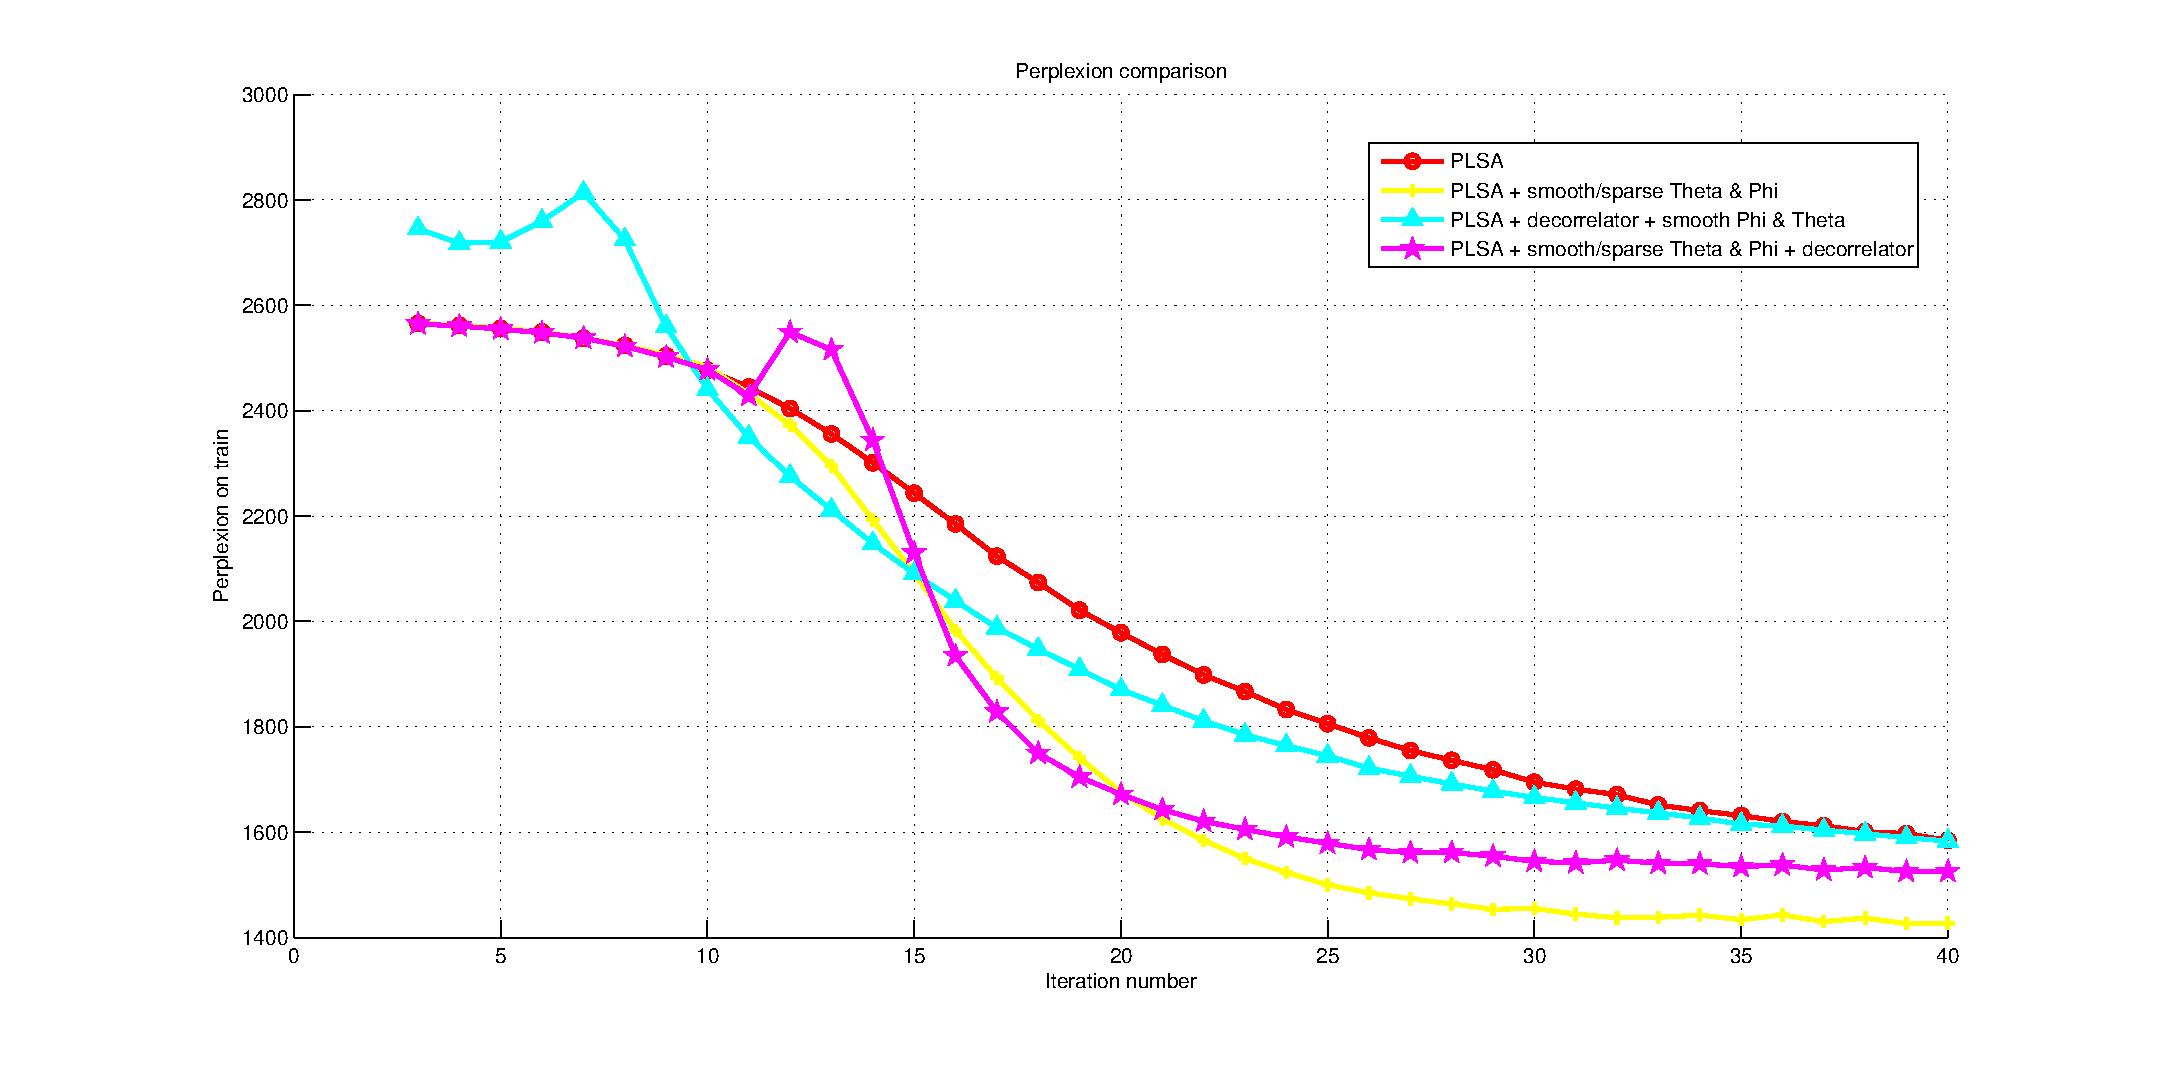
\includegraphics[scale = 0.5]{perplex.eps}
\caption{Ось X --- номер внешней итерации, ось Y --- перплексия моделей на обучающей выборке.}
\end{figure}

\begin{figure}[h!]\center
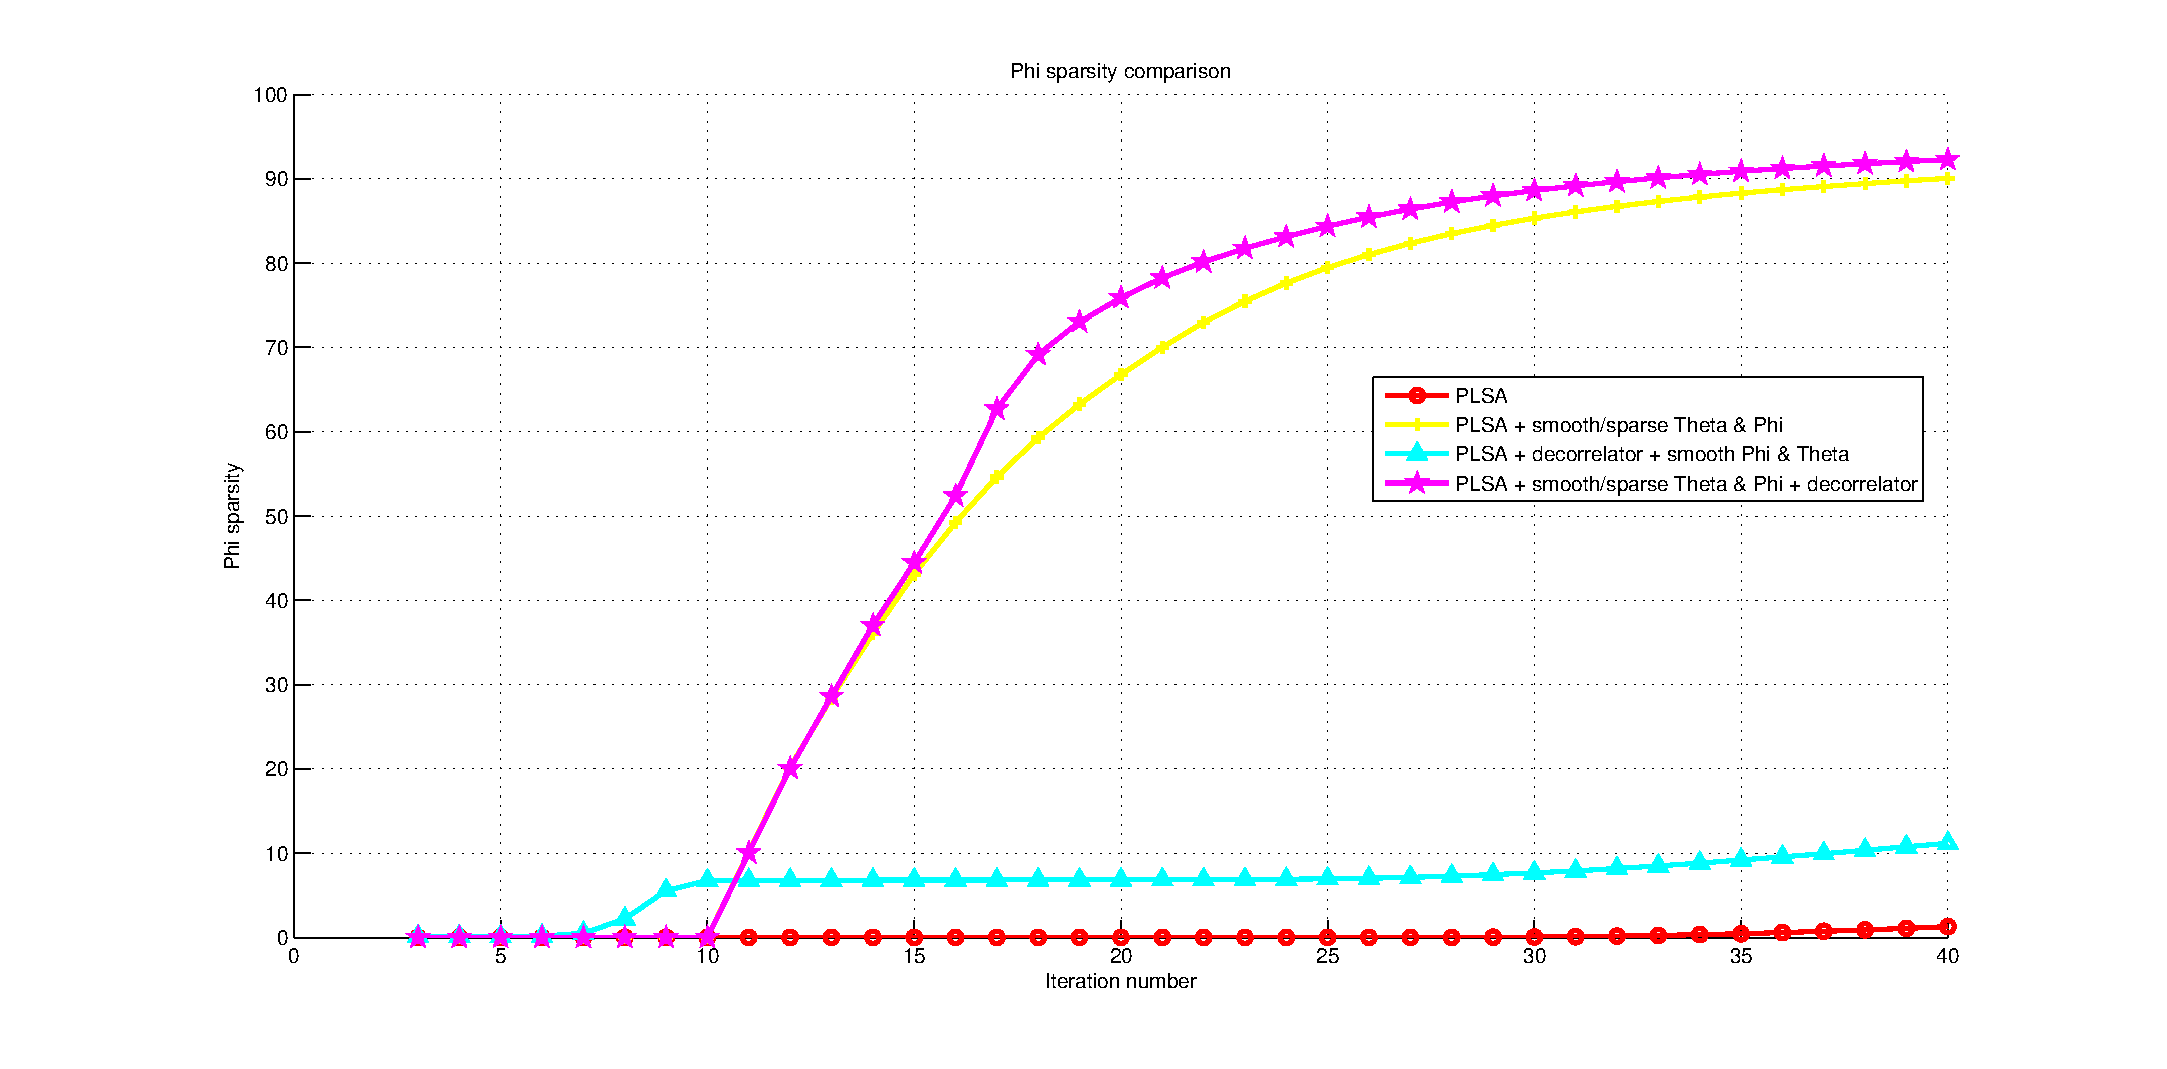
\includegraphics[scale = 0.5]{phi_sp.eps}
\caption{Ось X --- номер внешней итерации, ось Y --- разреженность матрицы $\Phi$ моделей.}
\end{figure}

\begin{figure}[h!]\center
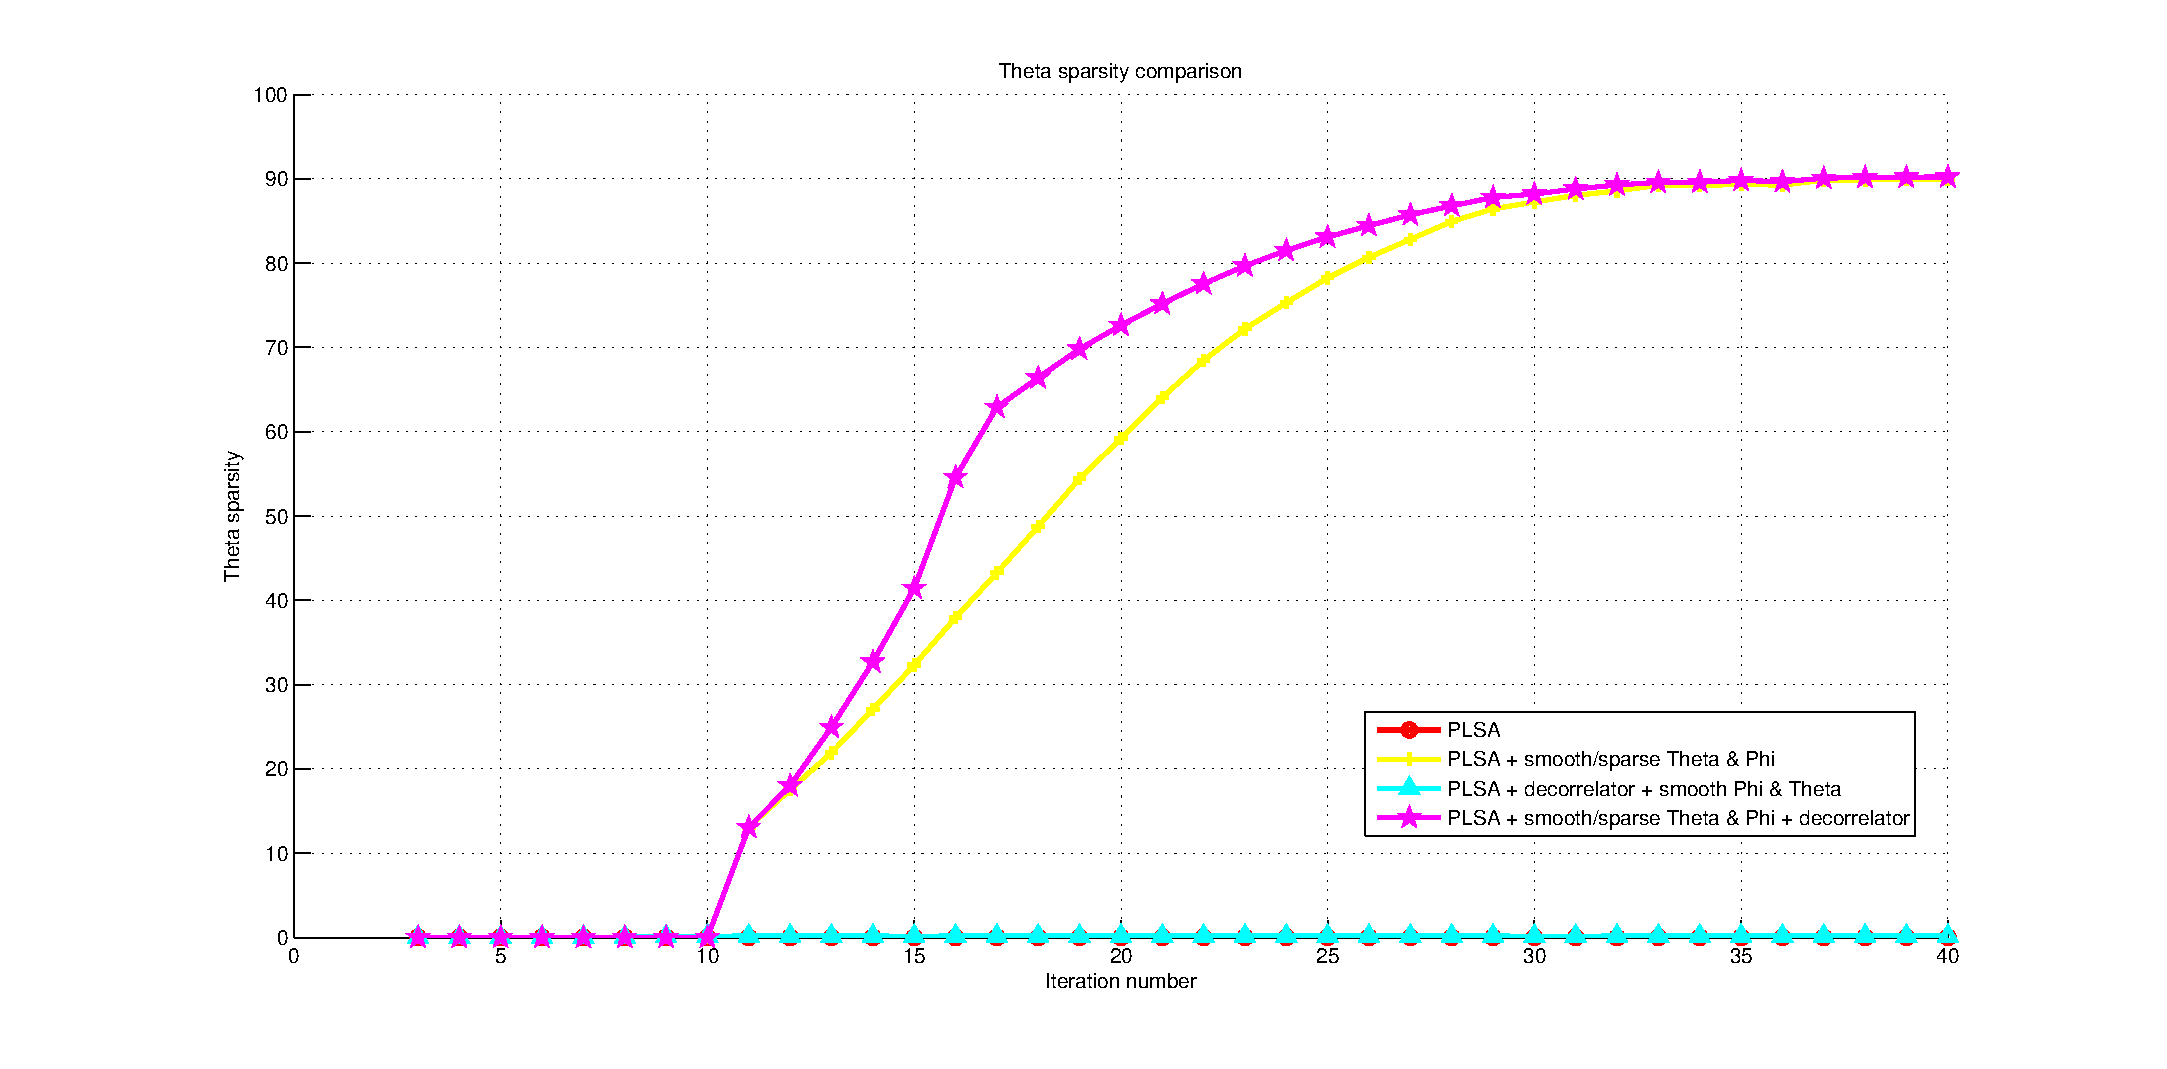
\includegraphics[scale = 0.5]{theta_sp.eps}
\caption{Ось X --- номер внешней итерации, ось Y --- разреженность матрицы $\Theta$ моделей.}
\end{figure}

\begin{figure}[h!]\center
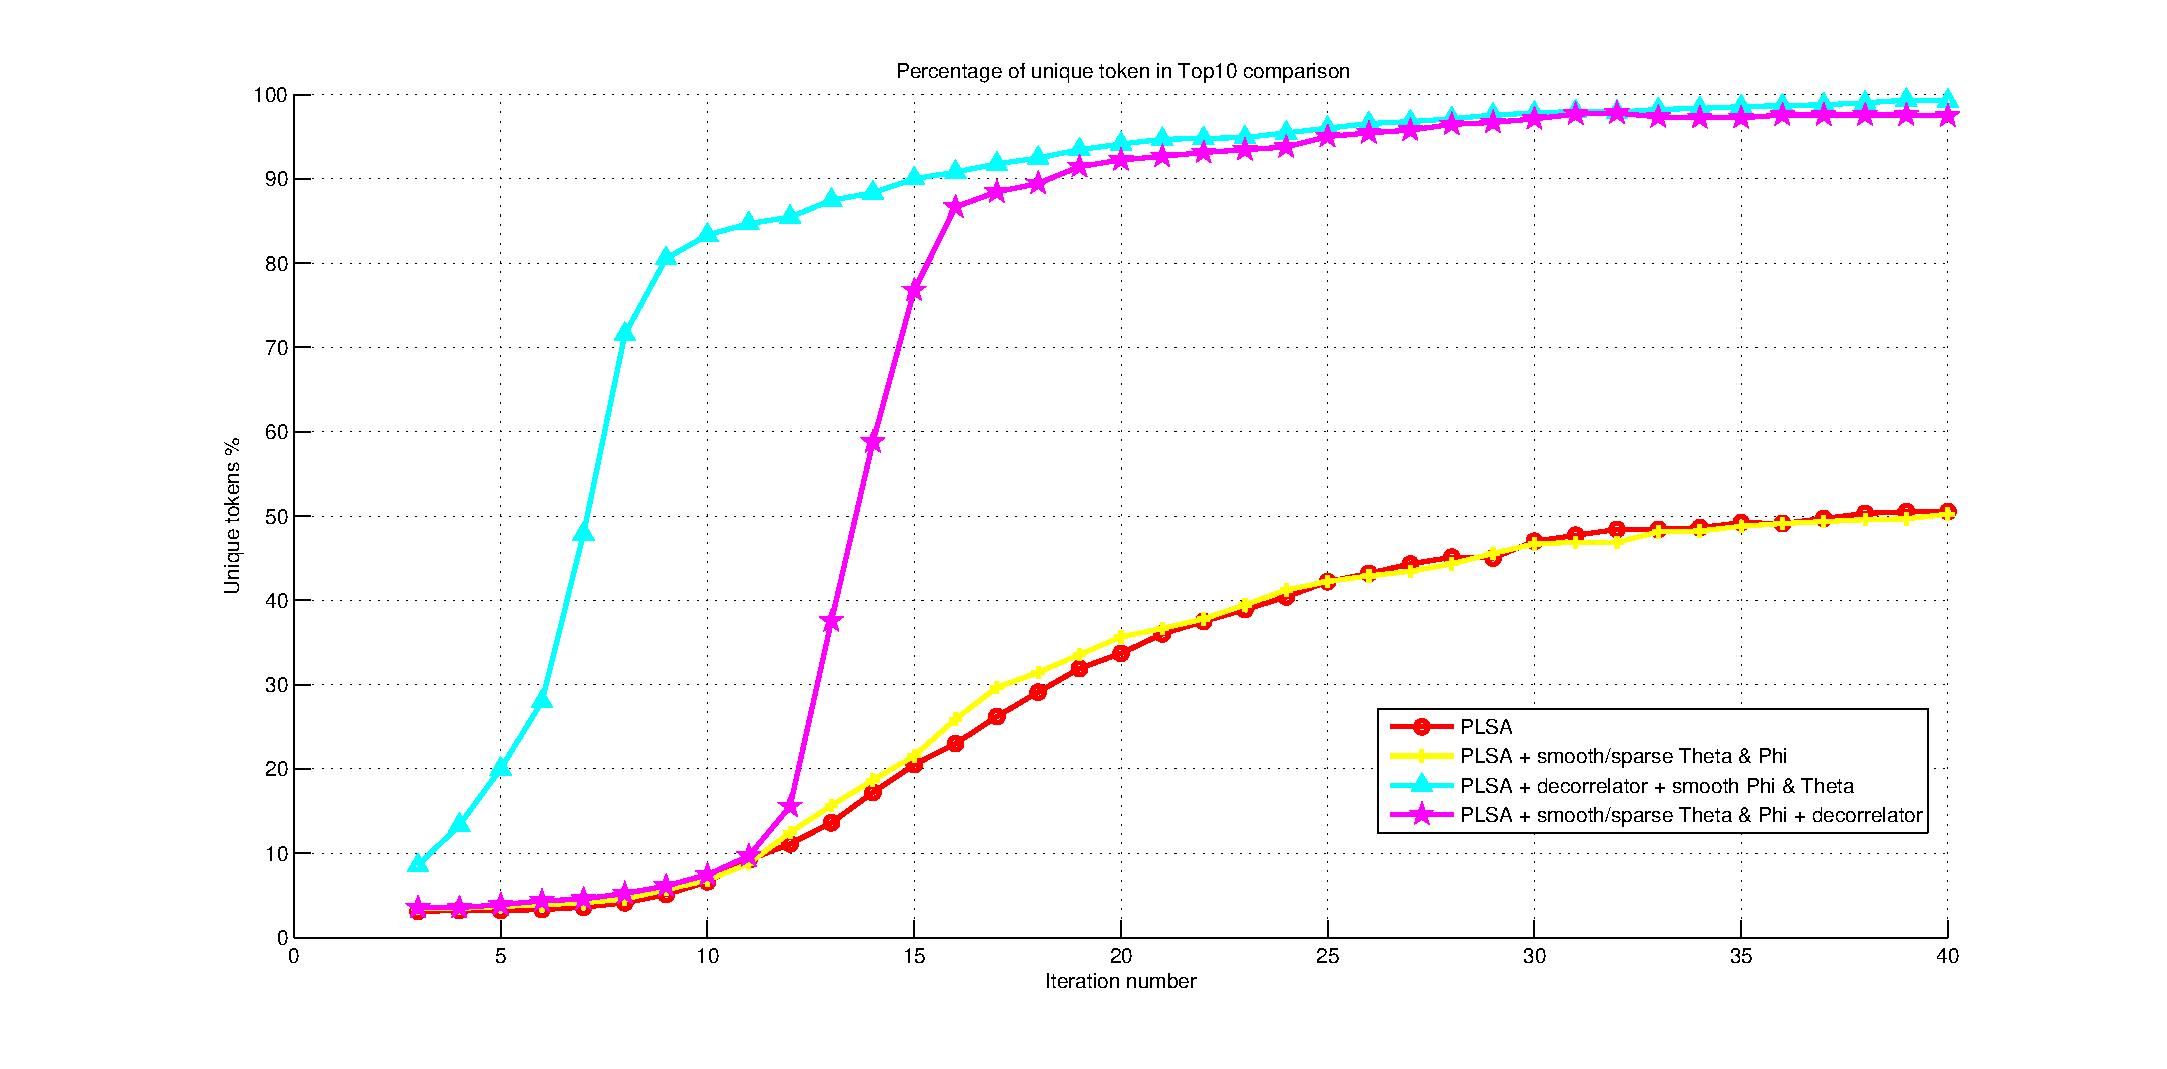
\includegraphics[scale = 0.5]{top10.eps}
\caption{Ось X --- номер внешней итерации, ось Y --- процент уникальных слов в Топ 10.}
\end{figure}

\begin{figure}[h!]\center
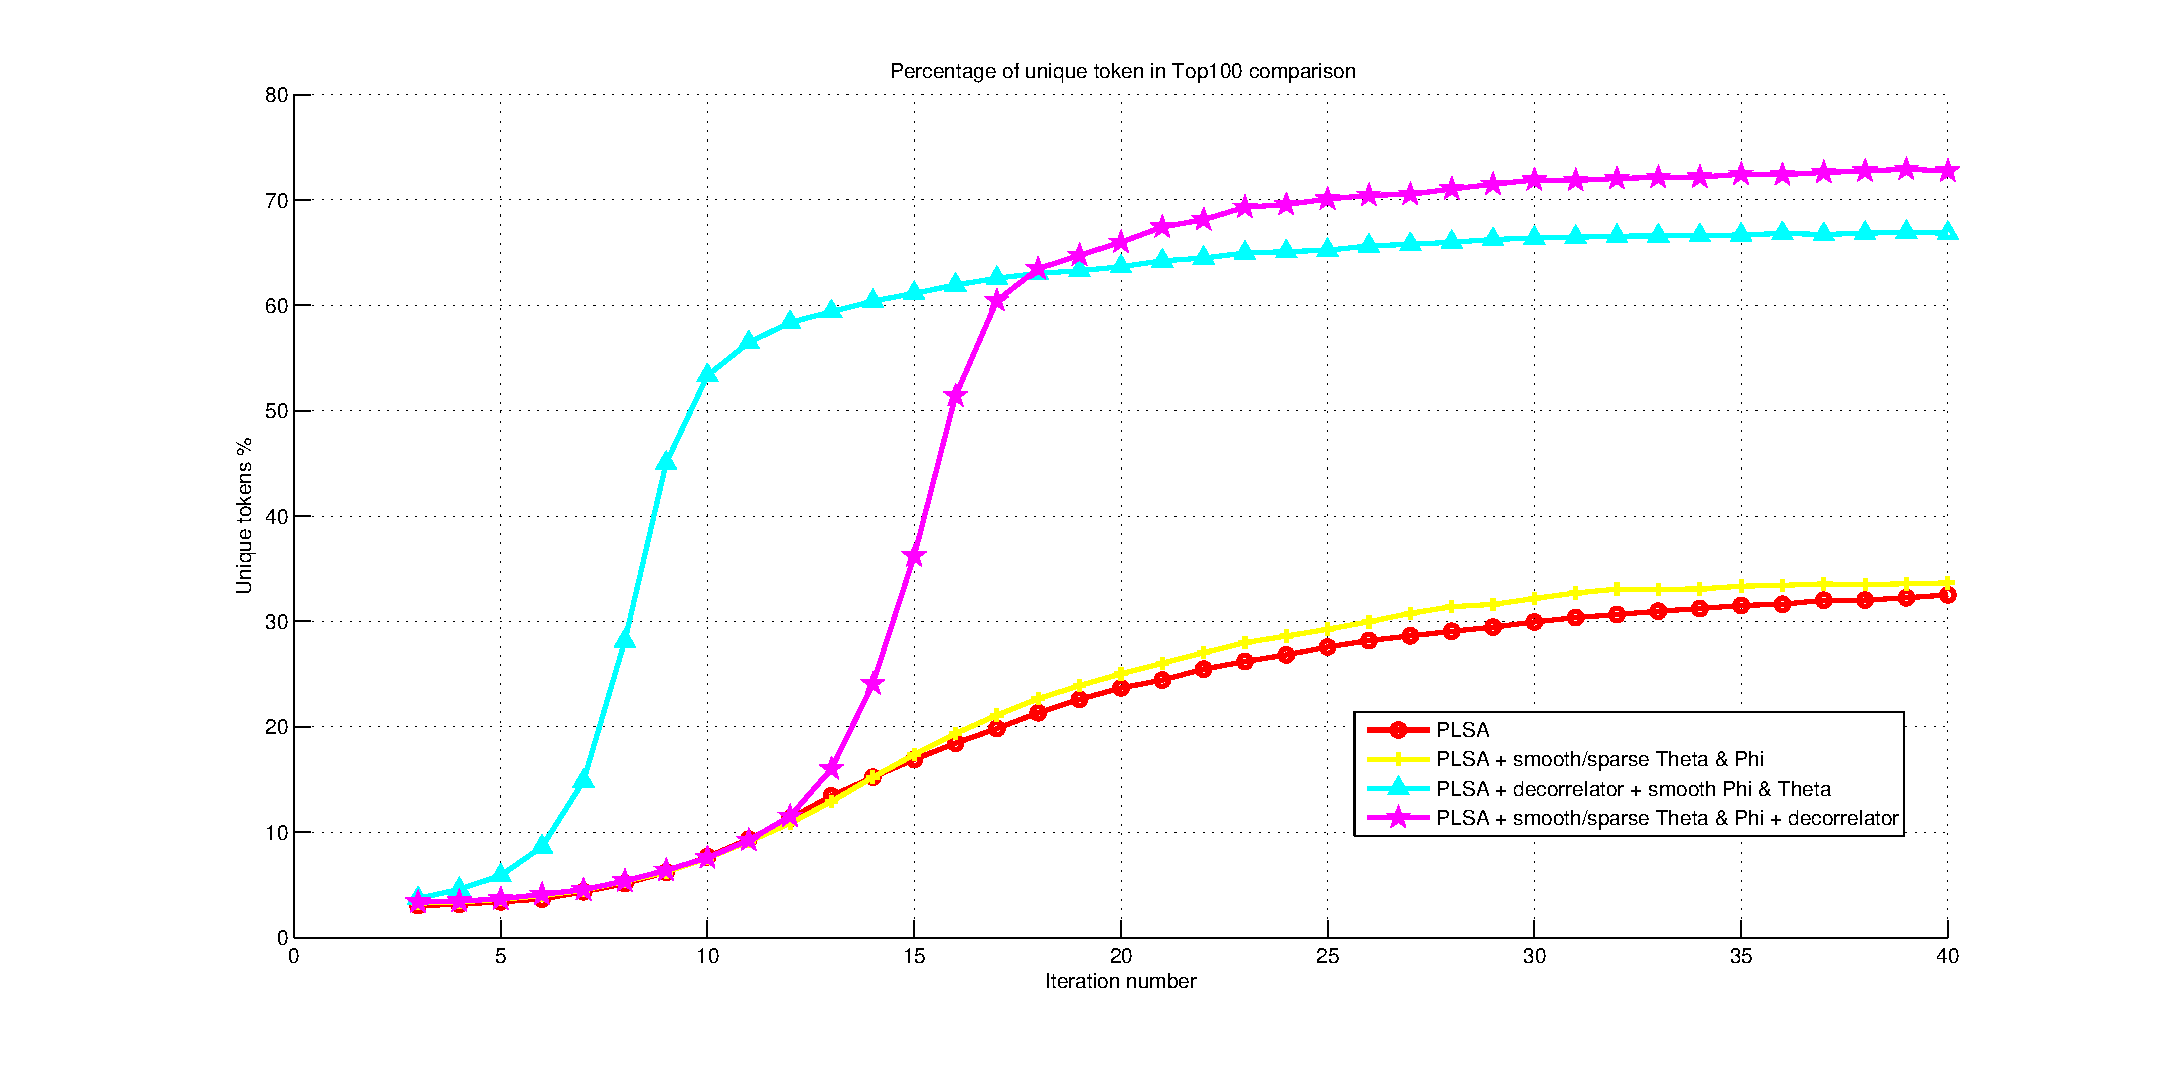
\includegraphics[scale = 0.5]{top100.eps}
\caption{Ось X --- номер внешней итерации, ось Y --- процент уникальных слов в Топ 100.}
\end{figure}

\section{Заключение}\label{results}
$\quad\;\:$Все задачи, поставленные перед данной курсовой работой, были выполнены. Был произведён обзор текущих возможностей BigARTM, перспективы её развития, описаны инструкции по работе с библиотекой. Кратко были рассмотрены существующие библиотеки тематического моделирования, их алгоритмические и архитектурные особенности, в т.ч. и нашедшие применение в BigARTM. 

В библиотеке BigARTM была создана и отлажена структура работы с регуляризаторами тематических моделей. Она была протестирована и доказала свою работоспособность. Были описаны примеры регуляризаторов, которые могут быть использованы как при решении реальных задач, так и в качестве основы для создания более сложных механизмов регуляризации.

Дальнейшая деятельность в рамках проекта по созданию библиотеки будет направлена на внедрение описанных в тексте работы планируемых нововведений.


\newpage
\addcontentsline{toc}{section}{Список литературы}
\begin{thebibliography}{00}

\bibitem{voron2014}
Воронцов К. В. Аддитивная регуляризация тематических моделей коллекций текстовых документов // Доклады РАН. 2014. — Т. 455., №3. 268–271.

\bibitem{hofmann_plsa}
T.~Hofmann Probabilistic latent semantic indexing // Proceedings of the 22nd annual international
ACM SIGIR conference on Research and development in information retrieval. — New York, NY,
USA: ACM,~1999. — Pp. 50–57.

\bibitem{protobuf} 
https://developers.google.com/protocol-buffers/docs/tutorials

\bibitem{ad_lda}
David Newman, Arthur Asuncion, Padhraic Smyth and Max Welling --- Distributed Algorithms for Topic Models, 2009.

\bibitem{plda}
Yi Wang, Hongjie Bai, Matt Stanton, Wen-Yen Chen and Edward Y.Chang --- PLDA: Parallel Latent Dirichlet Allocation for Large-Scale Applications, 2009.

\bibitem{y_lda}
A. J. Smola and S. Narayanamurthy --- An architecture for parallel topic models, 2010.

\bibitem{plda_plus}
Liu, Z., Zhang, Y., Chang, E. Y., and Sun, M. --- PLDA+: Parallel Latent Dirichlet Allocation with Data Placement and Pipeline Processing, 2011.

\bibitem{voron_potap_14} 
Воронцов~К.В., Потапенко~А.А. --- Аддитивная регуляризация тематических моделей,~2014.

\end{thebibliography}

\end{document}
